\documentclass[12pt,ngerman,parskip=half,bibliography=totoc,titlepage]{scrreprt}
\usepackage[a4paper, left=3.5cm, right=2.5cm, top=2.5cm, bottom=2.5cm]{geometry}
\usepackage[utf8]{inputenc}
\usepackage[T1]{fontenc}
\usepackage[ngerman]{babel}
\usepackage{csquotes}
\usepackage{graphicx}
\usepackage{amsmath}
\usepackage{tabularx}
\usepackage{longtable}
\usepackage{float}
\usepackage{mathpazo}
% \usepackage{ebgaramond}
\usepackage[
  backend=biber,
  style=authoryear,
  citestyle=authoryear
]{biblatex}
\addbibresource{literatur.bib}
\usepackage{setspace} 
\onehalfspacing
\usepackage[hidelinks]{hyperref}

\begin{document}

\begin{titlepage}
  
\includegraphics[width=4cm]{images/hochschule_logo.png}\par\vspace{2cm}
  Facharbeit \newline \newline \newline
  {\large\textbf{Progressive Web App für Studierende: Eine App zur Verwaltung von Vorlesungen, Notizen und Prüfungen}}\\[1cm]
  im Studiengang\\
  Softwaretechnik und Medieninformatik (B. Eng)\newline \newline \newline
  vorgelegt von\newline \newline
    \textbf{Esra Balci}\\
    Matr.-Nr.: 766561\\
    E-Mail: esbait01@hs-esslingen.de\\
    am 24.06.2025\\ 
    an der Hochschule Esslingen \newline \newline
    \vspace{2ex} % Abstand unter der Linie
    \noindent\makebox[\textwidth]{\rule{\textwidth}{0.5pt}}
    \vspace{2ex}
    {\textbf{Prüferin: Prof. Dipl.-Informatikerin Astrid Beck \\
    Zweitprüfer: Prof. Dr.-Ing. Harald Melcher
    }}

\end{titlepage}

\tableofcontents

\cleardoublepage
\phantomsection
\addcontentsline{toc}{chapter}{Abbildungsverzeichnis}
\listoffigures

\cleardoublepage
\phantomsection
\addcontentsline{toc}{chapter}{Tabellenverzeichnis}
\listoftables

\cleardoublepage

\chapter{Einleitung}
\section{Motivation und Zielsetzung}
In einer Zeit, in der das digitale Studium stetig an Bedeutung gewinnt, stehen Studierende vor der Herausforderung, eine Vielzahl an Terminen und Materialien effizient zu verwalten. Handschriftliche Notizen sowie verstreute Kalendereinträge verursachen häufig Unübersichtlichkeit und Stress.\newline 
Mit der zunehmenden Digitalisierung steigt der Bedarf an eigenverantwortlicher Organisation des Lernalltags. Studien zeigen, dass Selbstorganisations- und Motivationsfähigkeiten zentrale Voraussetzungen für erfolgreiches Arbeiten und Lernen sind - insbesondere in agilen und digitalen Umgebungen \autocite{selbstorganisation}. Gerade für Studierende bedeutet das, geeignete Werkzeuge zu nutzen, um Termine, Inhalte und Notizen effizient zu strukturieren. Die im Rahmen dieser Arbeit entwickelte Web App adressiert genau diese Bedürfnisse. \newline \newline
Ziel ist es, eine Progressive Web App (PWA) zu entwickeln, die nicht nur Vorlesungspläne und Termine in einer übersichtlichen Oberfläche bündelt, sondern auch das Anlegen und Wiederfinden persönlicher Notizen erleichtert. Dabei stehen eine gebrauchstaugliche Bedienung, Offline-Funktionalität sowie eine nahtlose Synchronisierung über verschiedene Endgeräte hinweg im Fokus. Die Anwendung soll Studierende dabei unterstützen, ihren Studienalltag effizienter zu strukturieren und sich auf das Wesentliche - das Lernen - zu konzentrieren.

\section{Projektgegenstand}
Der Gegenstand dieses Projekts ist die Konzeption und Umsetzung einer PWA für Studierende, die drei Kernmodule integriert:
\begin{enumerate}
  \item \textbf{Vorlesungsmanagement}, das Stundenpläne visuell darstellt.
  \item \textbf{Kalender}, der Termine anzeigt.
  \item \textbf{Notizmodul}, das das Erstellen, Kategorisieren und Durchsuchen von persönlichen Lernnotizen ermöglicht.
\end{enumerate}
Die technologische Basis bildet ein ReactJS-Frontend, das PWA-Features nutzt, sowie ein in Node.js entwickeltes Backend, das in Docker-Containern läuft und eine MySQL-Datenbank verwaltet. Durch diese Architektur gewährleistet die Web App Skalierbarkeit, einfache Erweiterbarkeit und einen reibungslosen Betrieb in unterschiedlichen Hosting-Umgebungen.
\chapter{Anforderungen und Konzept}
\section{Zielgruppenanalyse}
Die Zielgruppe der Web App sind Studierende technischer und medienorientierter Studiengänge, die einen hohen Bedarf an Selbstorganisation haben. Viele verwenden mehrere Tools wie Papierkalendar, Notizapps, Moodle oder Google Kalender. Die Web App soll eine zentrale und strukturierte Plattform zur Verfügung stellen.\newline \newline
Digital unterstützte Selbstorganisation durch Studierende wird zunehmend international adressiert. \textcite{obexer} zeigen, dass die Rolle sogenannter Learning Designers - als Brücke zwischen Technologie und didaktischem Einsatz - nicht nur Lehrende unterstützt, sondern auch Studierende in ihrem Lernprozess stärkt. Sie betonen, dass ohne gezielte Support-Strukturen digitale Tools oft fragmentiert und ineffizeint genutzt werden. 
\section{Funktionale Anforderungen}
Die Progressive Web App soll die folgenden zentralen Funktionen bereitstellen:

\begin{itemize}
  \item \textbf{Vorlesungsverwaltung:} Nutzer:innen sollen Vorlesungen hinzufügen, bearbeiten und löschen können.
  \item \textbf{Kalenderintegration:} Prüfungstermine, Abgabefristen und Veranstaltungen sollen im Kalender sichtbar und verwaltbar sein.
  \item \textbf{Notizmodul:} Studierende sollen in der Lage sein, Notizen zu Vorlesungen zu speichern, zu verschlagworten und gezielt zu durchsuchen.
  \item \textbf{Offline-Funktionalität:} Die Anwendung soll auch ohne Internetzugang nutzbar bleiben (PWA-Standard).
  \item \textbf{Synchronisation:} Daten sollen geräteübergreifend synchronisiert werden.
  \item \textbf{Gebrauchstaugliche Oberfläche:} Die Web App soll eine intuitive, barrierearme Oberfläche bieten.
\end{itemize}
\section{User Stories}
Als Student:in möchte ich meine Vorlesungen eintragen, um meinen Stundenplan digital zu organisieren.\\
Als Student:in möchte ich Notizen zu Vorlesungen speichern, um diese später leicht und schnell zufinden.\\
Als Student:in ohne Internetverbindung möchte ich meine Notizen offline einsehen können, damit ich auch unterwegs lernen kann.\\
Als Student:in möchte ich Prüfungstermine in einem Kalender verwalten, um keine Fristen zu verpassen.

\section{Grobkonzept und Mock-ups}
Die Abblindung \ref{fig:homepage} zeigt die Startseite der Web App, die eine Übersicht über alle Vorlesungen und anstehenden Termine bietet. Die Navigation ermöglicht den Zugriff auf den Stundenplan, Notizen und den Kalender.
\begin{figure}[H]
  \centering
  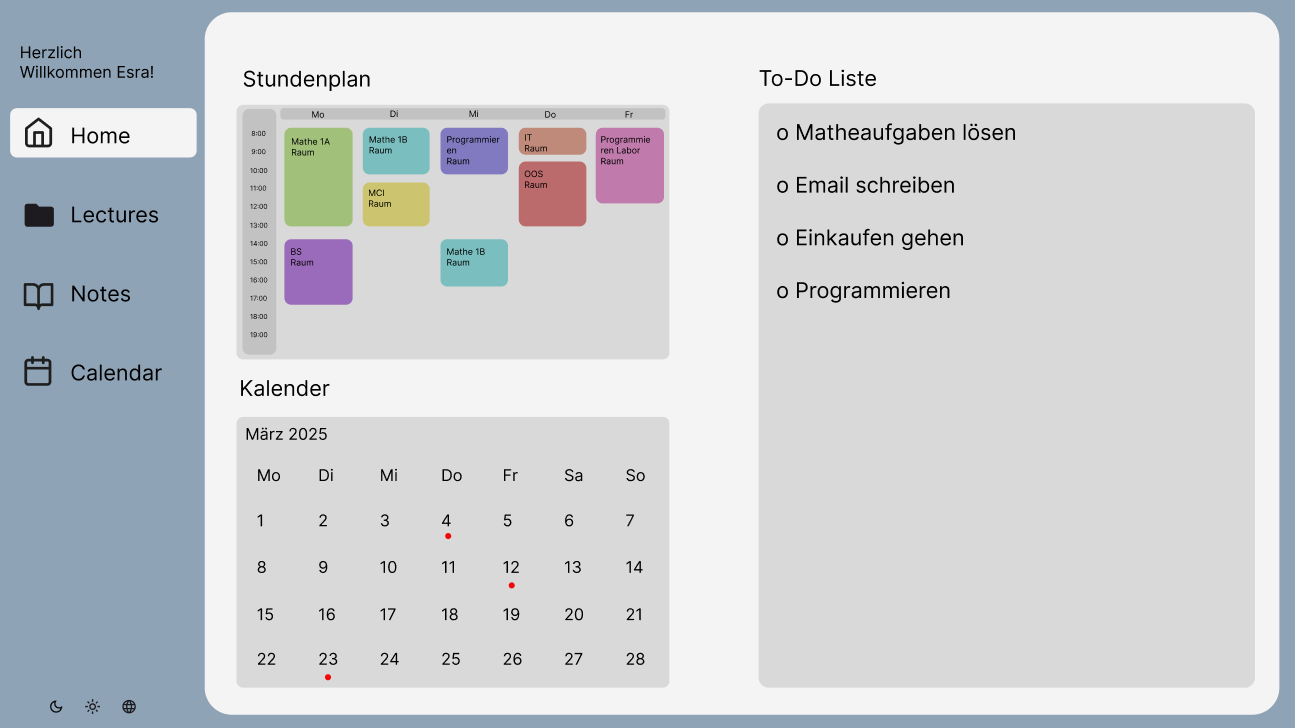
\includegraphics[width=1\textwidth]{./images/homepage.png}
  \caption{Startseite}
  \label{fig:homepage}
\end{figure}
In Abbildung \ref{fig:lectures} ist die Seite für die Verwaltung vom Stundenplan dargestellt. Hier können Nutzer:innen Vorlesungen hinzufügen, bearbeiten und löschen.
\begin{figure}[H]
  \centering
  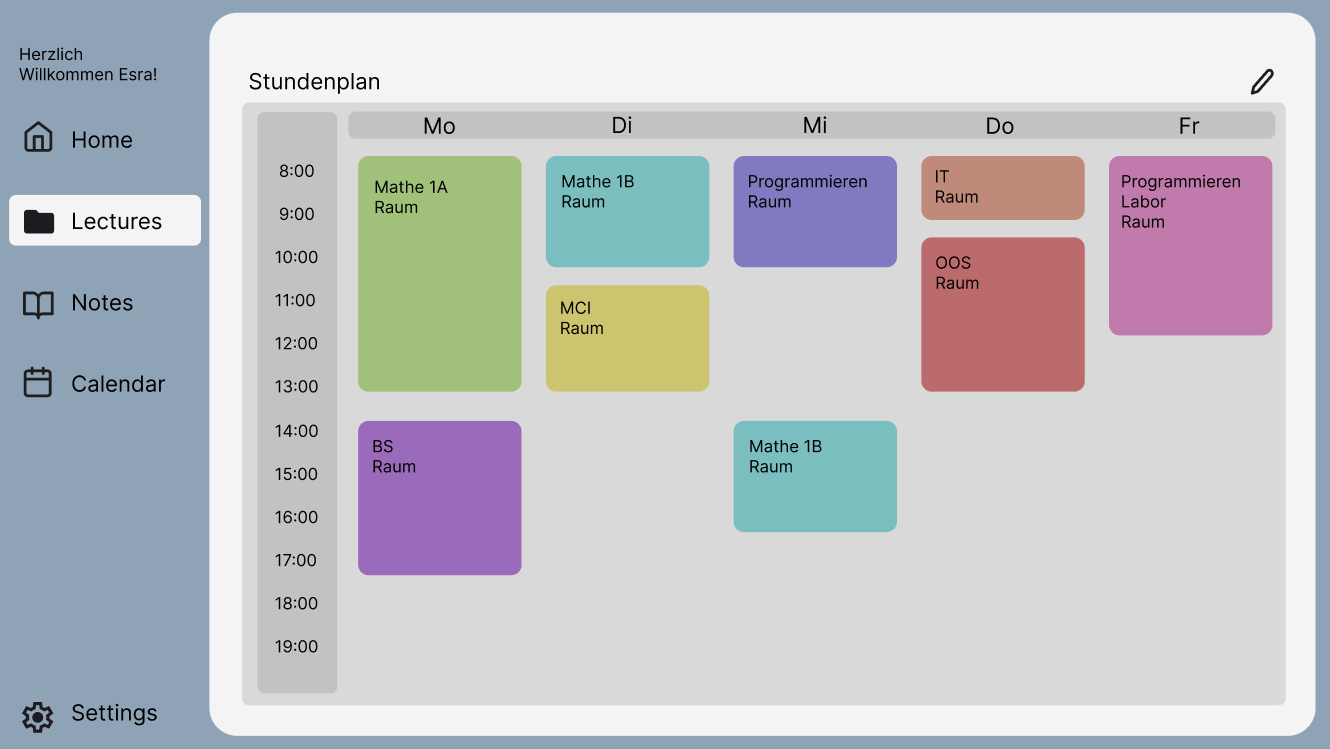
\includegraphics[width=1\textwidth]{./images/lecturepage.png}
  \caption{Stundenplan}
  \label{fig:lectures}
\end{figure}
 Die Abbildung \ref{fig:notes} zeigt das Notizmodul, in dem Studierende ihre Lernmaterialien organisieren können.
\begin{figure}[H]
  \centering
  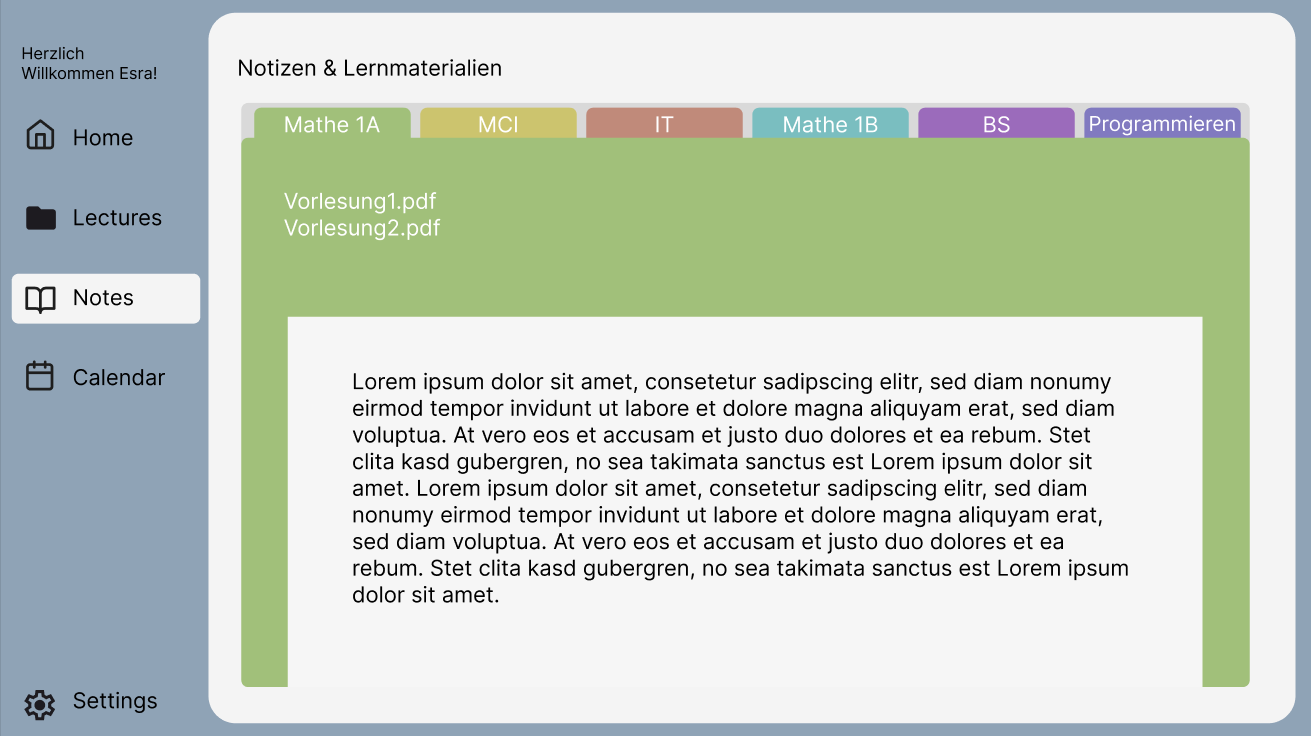
\includegraphics[width=1\textwidth]{./images/notespage.png}
  \caption{Notizen und Lernmaterialien}
  \label{fig:notes}
\end{figure}
Abbildung \ref{fig:calendar-1} und \ref{fig:calendar-2} zeigen den Kalender, in dem Prüfungstermine und Fristen eingetragen werden können. Nutzer:innen können neue Einträge hinzufügen und bestehende verwalten.
\begin{figure}[H]
  \centering
  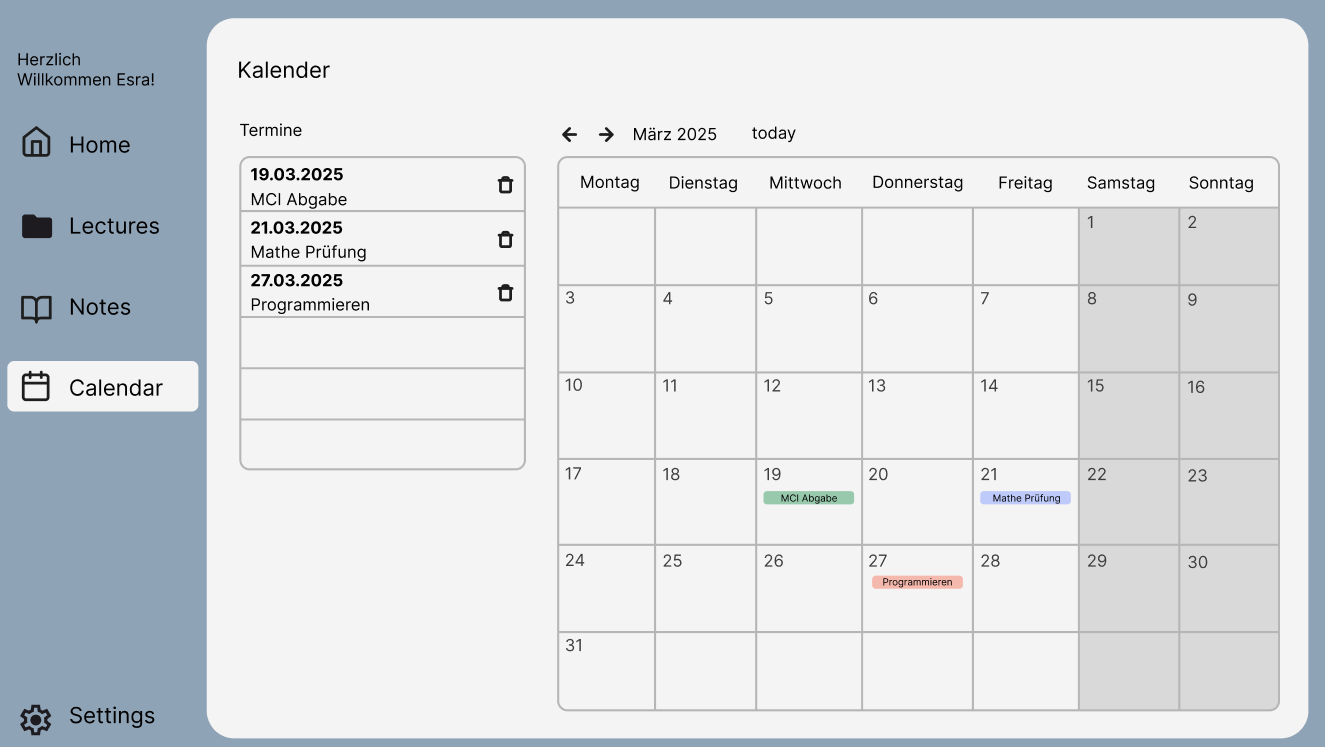
\includegraphics[width=1\textwidth]{./images/calendarpage-1.png}
  \caption{Kalender}
  \label{fig:calendar-1}
\end{figure}

\begin{figure}[H]
  \centering
  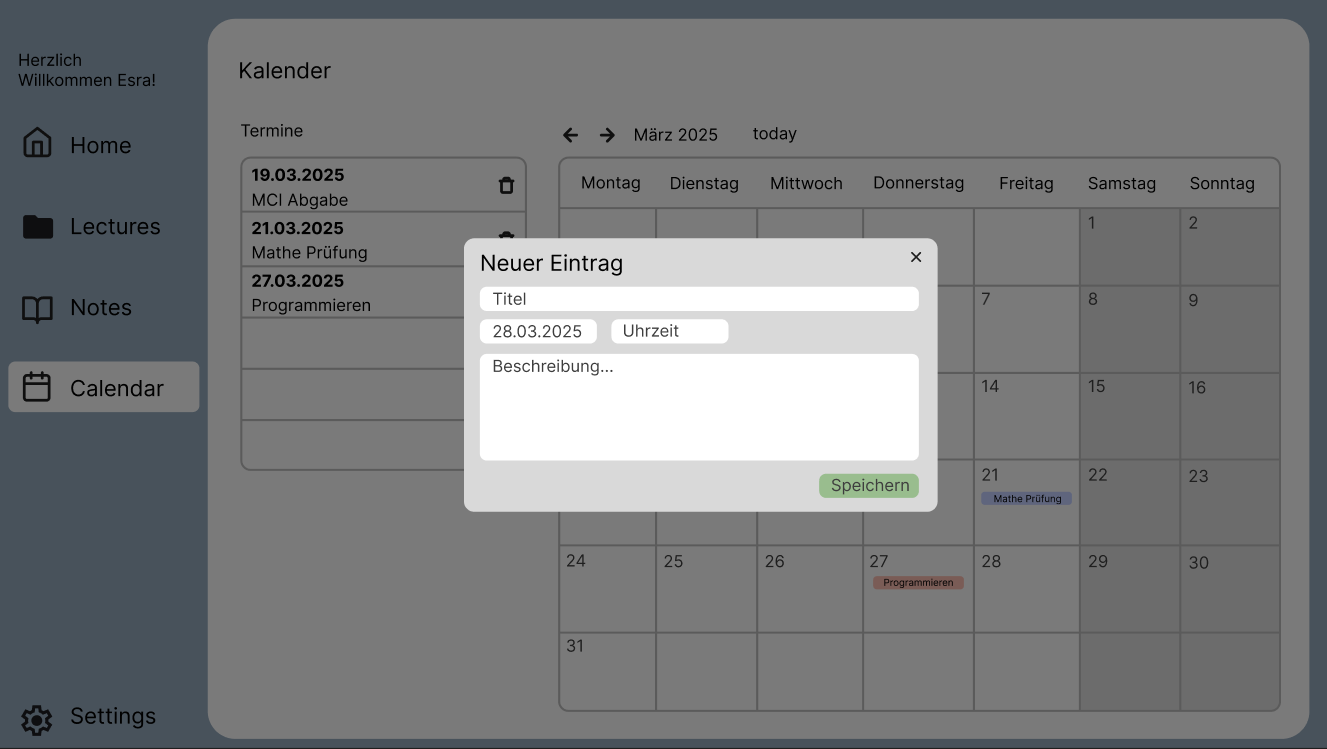
\includegraphics[width=1\textwidth]{./images/calendarpage-2.png}
  \caption{Neuen Eintrag in den Kalender einfügen}
  \label{fig:calendar-2}
\end{figure}
\chapter{Architekturübersicht}
\section{Gesamtsystem und Komponenten}
Das entwickelte System basiert auf einer modularen client-server-Architektur, bei der verschiedene Komponenten logisch getrennt, aber technisch eng miteinander verknüpft agieren. Ziel ist es, eine wartbare, skalierbare und plattformunabhängige Anwendung bereitzustellen, die sich durch hohe Gebrauchstauglichkeit auszeichnet.
\begin{itemize}
    \item \textbf{Frontend (Client):} Das Frontend ist als Single Page Application (SPA) mit ReactJS umgesetzt. Es bietet die Benutzeroberfläche für Studierende und ermöglicht das Erstellen und Anzeigen von Vorlesungen, Notizen, Kalenderereignissen und To-Dos. Das Frontend greift über HTTP auf die REST-API des Backends zu.
    \item \textbf{Backend:} Das Backend ist in Node.js realisiert und stellt eine RESTful API bereit, die die Geschäftslogik der Anwendung kapselt. Es verarbeitet Anfragen vom Frontend, kommuniziert mit der Datenbank und führt die erforderlichen Operationen aus. Durch die Containerisierung in Docker ist eine konsistente Ausführung in verschiedenen Umgebungen gewährleistet.
    \item \textbf{Datenbank:} Die persistenten Daten werden in einer MySQL-Datenbank gespeichert. Diese läuft als Container innerhalb der Entwicklungs- und Produktionsumgebung. Die Datenbank enthält strukturierte Informationen zu Vorlesungen, Notizen, Kalenderereignissen und Stundenplaneinträgen. Das relationale Datenmodell erlaubt eine logische Trennung der Entitäten und eine effiziente Verarbeitung auch großer Datenmengen.
    \item \textbf{Dateispeicherung:} Hochgeladene Datein (z.B. PDF-Dokumente im Notizmodul) werden im lokalen Uploads-Verzeichnis des Servers gespeichert. Dieses Verzeichnis wird über einen statischen Pfad (/uploads) öffentlich bereitgestellt.
\end{itemize}
\section{Technologiestack}
In diesem Abschnitt werden die verwendeten Technologien beschrieben.
\subsection{ReactJS}
React ist eine Open-Source-JavaScript-Bibliothek, die dem User ermöglicht, Benutzeroberflächen aus einzelnen, wiederverwendbaren Komponenten zu erstellen. Mit React lassen sich sowohl klassische Web-UIs als auch native Benutzeroberflächen für Mobil- und Desktop-Apps realisieren, indem die gleichen Konzepte und das gleiche API-Design genutzt werden, so bleibt der Workflow plattformübergreifend konsistent und effizient. \autocite{react}
\subsection{PWA}
Eine Progressive Web App (PWA) ist eine Webanwendung, die moderne Webtechnologien wie HTML, CSS und JavaScript nutzt, um das Nutzungserlebnis einer nativen mobilen App nachzuahmen. Dabei kann sie über einen gewöhnlichen Webbrowser aufgerufen werden, lässt sich jedoch auch wie eine klassische App auf dem Startbildschirm eines Geräts installieren. PWAs zeichnen sich durch Eigenschaften wie Offline-Funktionalität, schnelle Ladezeiten, Push-Benachrichti-gungen und eine für mobile Endgeräte optimierte Benutzeroberfläche aus. Ziel ist es, die Vorteile von Websites mit denen nativer Apps zu kombinieren und somit eine plattformübergreifende, gebrauchstaugliche Lösung bereitzustellen. \autocite{pwa}
\subsection{Node.js}
Node.js ist eine offene, plattformübergreifende JavaScript-Laufzeitumgebung, die es ermöglicht, JavaScript nicht nur im Browser, sondern auch auf Servern, in Kommandozeilen-Tools und Skripten einzusetzen. Node.js bietet Entwicklern eine moderne, ereignisorientierte Plattform zur Erstellung hochskalierbarer Netzwerkapplikationen, ohne komplexe Thread-Verwaltung oder Blocking-I/O-Pro-bleme. \autocite{nodejs}
\subsection{MySQL}
MySQL ist ein weit verbreitetes, quelloffenes relationales Datenbankmanagementsystem (RDBMS). Es speichert strukturierte Daten in Tabellen mit expliziten Zeilen und Spalten, die durch Schemata definiert sind. Abfragen und Manipulation erfolgen über die standardisierte Sprache SQL (Structured Query Language). MySQL unterstützt ACID-konforme Transaktionen, was für sichere und zuverlässige Datenverarbeitung sorgt. Dank seiner hohen Leistung, Skalierbarkeit und der großen Entwickler-Community eignet sich MySQL sowohl für kleine Anwendungen als auch für internationale Webseiten, Webdienste und Unternehmenssysteme. \autocite{mysql}
\subsection{Docker}
Docker ist eine Plattform für Betriebssystemvirtualisierung, die Anwendungen in sogenannten Containern verpackt. Diese Container enthalten nicht nur die Anwendung selbst, sondern auch alle benötigten Abhängigkeiten. Im Gegensatz zu VMs teilen sich Container den Kernel des Host-Systems, was sie deutlich leichter und schneller macht. Images dienen dabei als Bauvorlagen und Container laufen als deren Instanzen. Docker unterstützt eine konsistente Portabilität über verschiedene Umgebungen hinweg und ermöglicht skalierbare, isolierte Anwendungsbereitstellung. Registry-Services wie Docker Hub erlauben das Teilen und Verwalten von Images. Zusätzlich bieten Tools wie Docker Compose die Orchestrierung mehrerer Container innerhalb komplexerer Anwendungen. \autocite{docker}
\section{Datenmodell und Datenbank}
Zur strukturierten und konsistenten Verwaltung der Anwendungsdaten wird ein relationales Datenmodell verwendet. Die Datenbank bildet das Rückgrat für die Speicherung von Informationen zu Vorlesungen, Notizen und Kalendereinträgen.\\
Zum Einsatz kommt eine MySQL-Datenbank, da dieses System weit verbreitet, gut dokumentiert und durch seine stabile Performance besonders geeignet für webbasierte Anwendungen ist. Die Datenbank läuft als eigenständiger Docker-Container und ist über eine REST-API mit dem Backend verbunden.\\
Für die Verwaltung und Speicherung der Anwendungsdaten wird eine relationale Datenbankstruktur verwendet, die mit MySQL umgesetzt wurde. Das Datenmodell ist in mehrere logisch getrennte Entitäten gegliedert und orientiert sich an den funktionalen Anforderungen der Webanwendung. Die folgende Grafik zeigt den schematischen Aufbau des Datenbanksystems:
\begin{figure}[H]
  \centering
  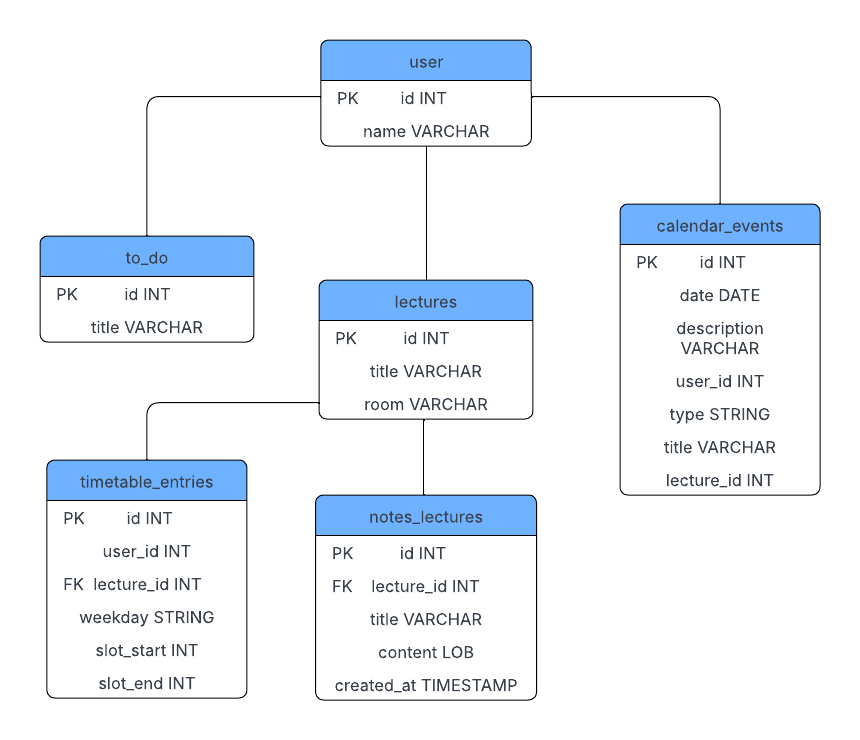
\includegraphics[width=1\textwidth]{./images/datenbankmodell.png}
  \caption{Datenbankmodell}
  \label{fig:datenbankmodell}
\end{figure}

\textbf{Entitäten und Beziehungen:}
\begin{itemize}
    \item \textbf{user:} Enthält Informationen zu den registrierten Nutzer:innen. Nutzer:innen können mehrere Vorlesungen, Notizen, Kalenderereignisse und To-Do-Einträ-ge besitzen.
    
    \item \textbf{lectures:} Repräsentiert einzelne Vorlesungen. Jede Vorlesung kann mit mehreren Notizen und Stundenplaneinträgen verknüpft sein.
    
    \item \textbf{notes\underline{ }lectures:} Speichert zu einer bestimmten Vorlesung gehörende Notizen mit Titel, Inhalt und Zeitstempel. Die Beziehung zu \texttt{lectures} erfolgt über einen Foreign Key.
    
    \item \textbf{calendar\underline{ }events:} Enthält Ereignisse wie Prüfungen, Abgaben oder Termine.
    
    \item \textbf{timetable\underline{ }entries:} Bildet konkrete Stundenplaneinträge ab. Neben der Vorle-sungs-ID werden auch Wochentag, Start- und Endzeit gespeichert.
    
    \item \textbf{to\underline{ }do:} Dient der Verwaltung einfacher Aufgabenlisten, die einem Nutzer:in-nen zugeordnet sind.
\end{itemize}
\textbf{Vorteile der Struktur:}
\begin{itemize}
    \item \textbf{Erweiterbarkeit:} Neue Funktionalitäten (z.B. Gruppen oder Tags) lassen sich durch zusätzliche Entitäten ohne größere Änderungen realisieren.
    \item \textbf{Skalierbarkeit:} Die klaren Beziehungen ermöglichen effiziente Abfragen, auch bei großen Datenmengen.
    \item \textbf{Wartbarkeit:} Die logische Trennung der Daten erhöht die Übersichtlichkeit und erleichtert Änderungen am Datenmodell.
\end{itemize}

\section{API-Design}
Die Kommunikation zwischen Frontend und Backend erfolgt über eine RESTful API, die auf dem HTTP-Protokoll basiert. Die Daten werden im JSON-Format übertragen. Die API stellt Endpunkte für die zentralen Funktionen der Anwendung bereit, wie das Erstellen und Abrufen von Vorlesungen, Notizen, Kalenderereignissen und Aufgaben.\\
\begin{longtable}{|p{6cm}|p{2cm}|p{6cm}|}
\hline
\textbf{Endpoint} & \textbf{Methode} & \textbf{Beschreibung} \\
\hline
/api/events & GET & Lädt alle Kalendereinträge, optional gefiltert nach \texttt{user\_id} und \texttt{type}. \\
\hline
/api/events & POST & Erstellt einen neuen Kalendereintrag mit Datum, Titel, Beschreibung usw. \\
\hline
/api/events/:id & DELETE & Löscht einen Kalendereintrag anhand seiner ID. \\
\hline
/api/lectures & GET & Gibt eine Liste aller Vorlesungen zurück. \\
\hline
/api/lectures & POST & Fügt eine neue Vorlesung mit Titel und Raum hinzu. \\
\hline
/api/lectures/:id & GET & Gibt eine bestimmte Vorlesung anhand ihrer ID zurück. \\
\hline
/api/lectures/:id & DELETE & Löscht eine Vorlesung anhand ihrer ID. \\
\hline
/api/timetable & POST & Fügt einen Stundenplaneintrag für einen bestimmten Nutzer hinzu. \\
\hline
/api/timetable/:user\_id & GET & Gibt den vollständigen Stundenplan eines Nutzers zurück. \\
\hline
/api/timetable/:id & DELETE & Löscht einen Stundenplaneintrag anhand seiner ID. \\
\hline
/api/to\_do & POST & Fügt einen neuen To-Do-Eintrag hinzu. \\
\hline
/api/to\_do & GET & Lädt alle To-Do-Einträge. \\
\hline
/api/to\_do/:id & DELETE & Löscht einen bestimmten To-Do-Eintrag. \\
\hline
/api/notes\_lectures & POST & Lädt eine neue Notiz zu einer Vorlesung hoch (PDF + Titel). \\
\hline
/api/notes\_lectures & GET & Lädt alle Notizen, sortiert nach Erstellungsdatum. \\
\hline
/api/notes\_lectures/:lecture\_id & GET & Lädt alle Notizen zu einer bestimmten Vorlesung. \\
\hline
/api/notes\_lectures/:id & DELETE & Löscht eine hochgeladene Notiz anhand ihrer ID. \\
\hline
\end{longtable}

Die grundsätzliche Systemarchitektur ist in Abbildung \ref{fig:systemarchitektur} dargestellt. Sie zeigt die Interatkion zwischen den drei Hauptkomponenten der Anwendung: dem ReactJS-basierten Frontend, dem containerisierten Node.js-Backend sowie der My-SQL-Datenbank. Die Kommunikation erfolgt dabei über standardisierte HTTP- und SQL-Schnittstellen. Auch der Prozess des Datei-Uploads ist visualisiert: Hochgeladene Dokumente werden vom Frontend an das Backend übermittelt und dort im Verzeichnis \texttt{/uploads} gespeichert, auf das wiederum das Frontend zur Anzeige zugreift.
\begin{figure}[H]
  \centering
  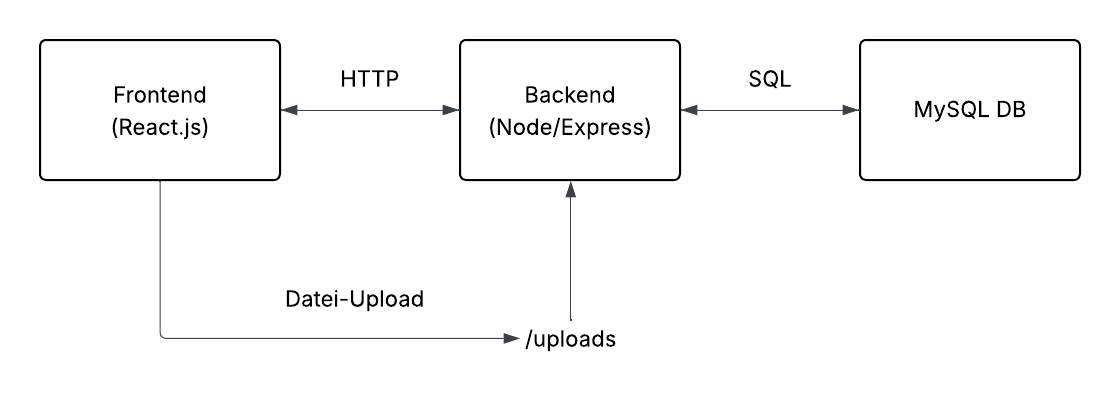
\includegraphics[width=1\textwidth]{./images/systemarchitektur.png}
  \caption{Systemarchitektur}
  \label{fig:systemarchitektur}
\end{figure}

% \chapter{Usability}
\chapter{Ergebnisse und Ausblick}
\section{Erreichte Funktionalitäten}

In Abbildung \ref{fig:startseite} ist die Startseite der WebApp zu sehen. Sie bietet eine Übersicht über die wichtigsten Funktionen und ermöglicht den schnellen Zugriff auf den Stundenplan, Notizen, Kalender und Einstellungen. Die Startseite ist so gestaltet, dass sie eine klare Navigation und eine ansprechende Benutzeroberfläche bietet.\newline
\begin{figure}[H]
  \centering
  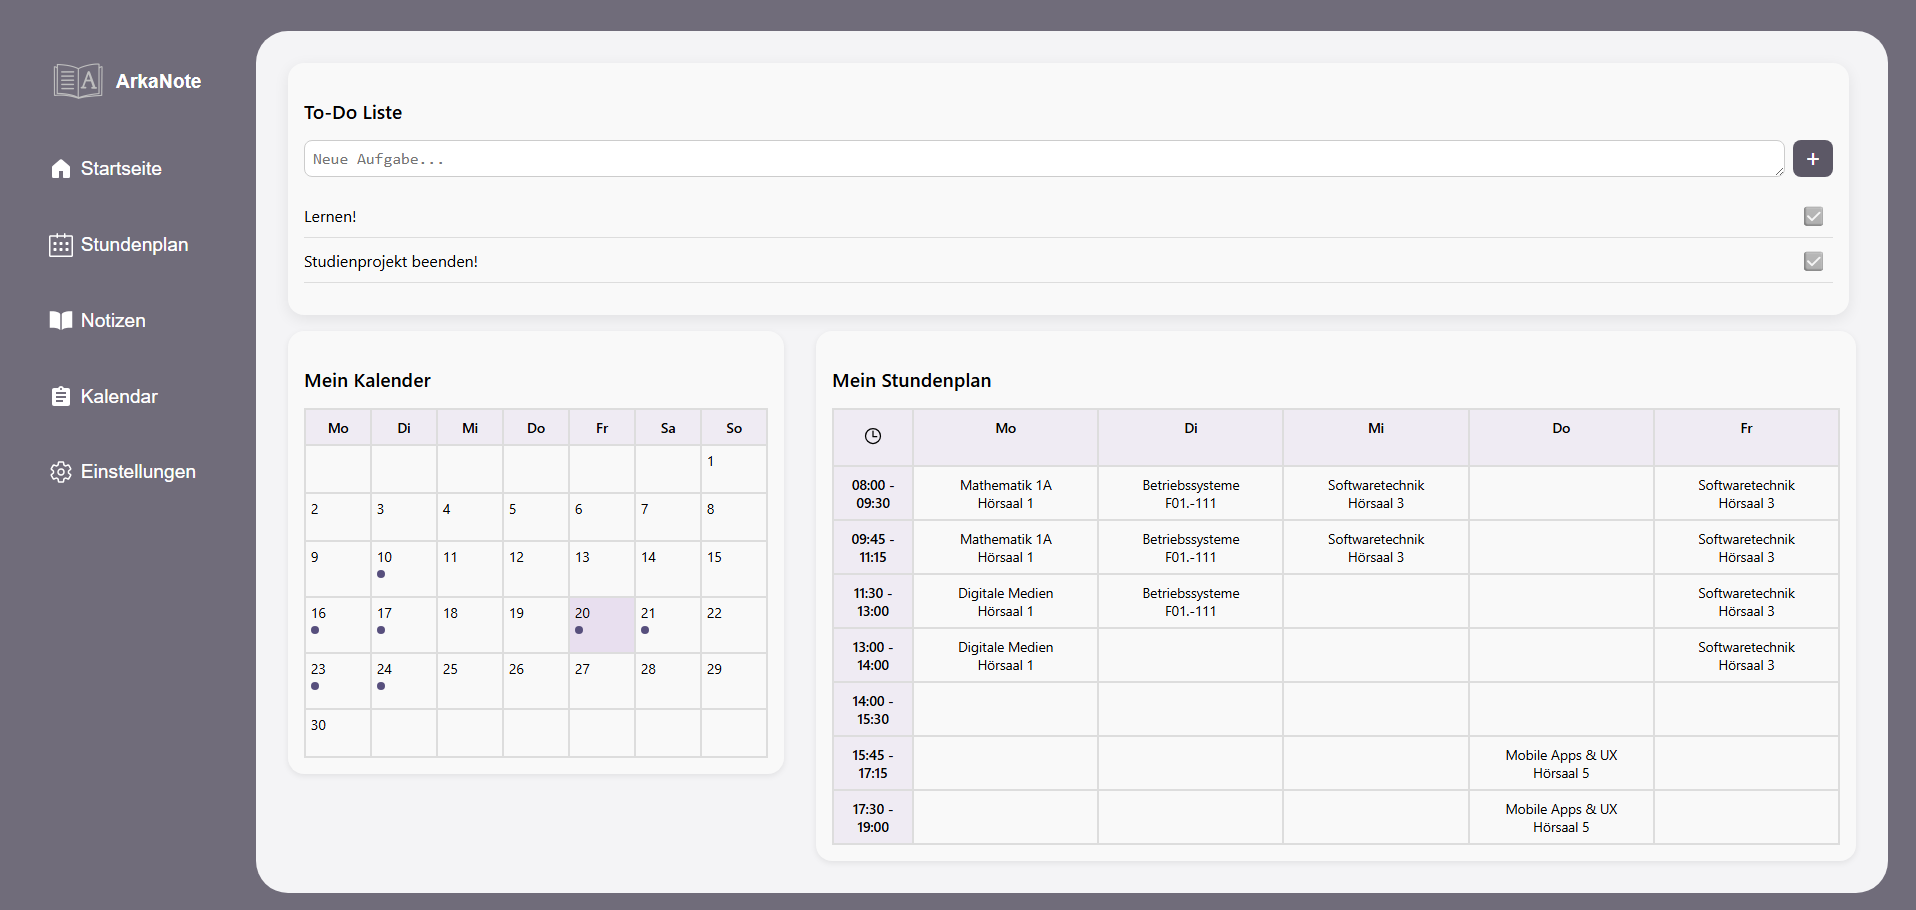
\includegraphics[width=1\textwidth]{./images/startseite.png}
  \caption{Startseite}
  \label{fig:startseite}
\end{figure}

Die WebApp ermöglicht es den Nutzer:innen, Vorlesungen zu verwalten und in ihren Stundenplan einzutragen. In Abbildung \ref{fig:stundenplan} ist der Stundenplan zu sehen, der eine visuelle Darstellung der Vorlesungen bietet. Nutzer:innen können neue Vorlesungen hinzufügen, wie in Abbildung \ref{fig:neue-vorlesungen} gezeigt, und diese dann in ihren Stundenplan eintragen (Abbildung \ref{fig:stundenplan-vorlesung}).\newline
\begin{figure}[H]
  \centering
  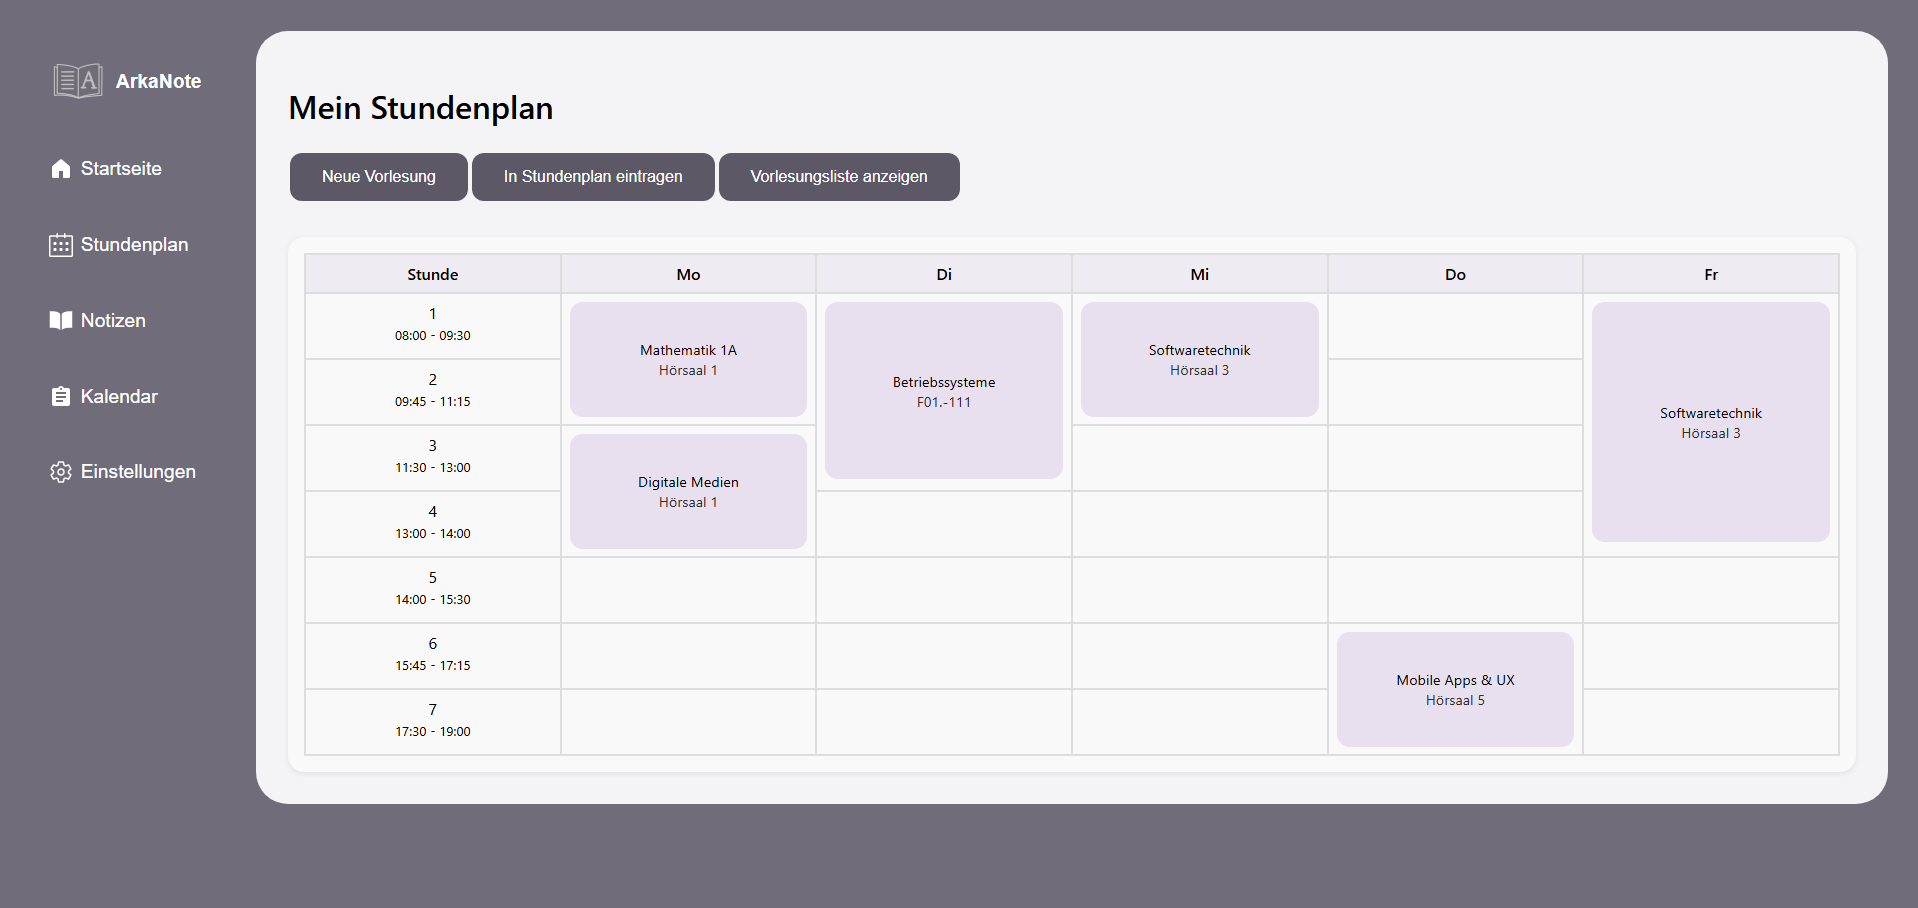
\includegraphics[width=1\textwidth]{./images/stundenplan.png}
  \caption{Stundenplan}
  \label{fig:stundenplan}
\end{figure}

\begin{figure}[H]
  \centering
  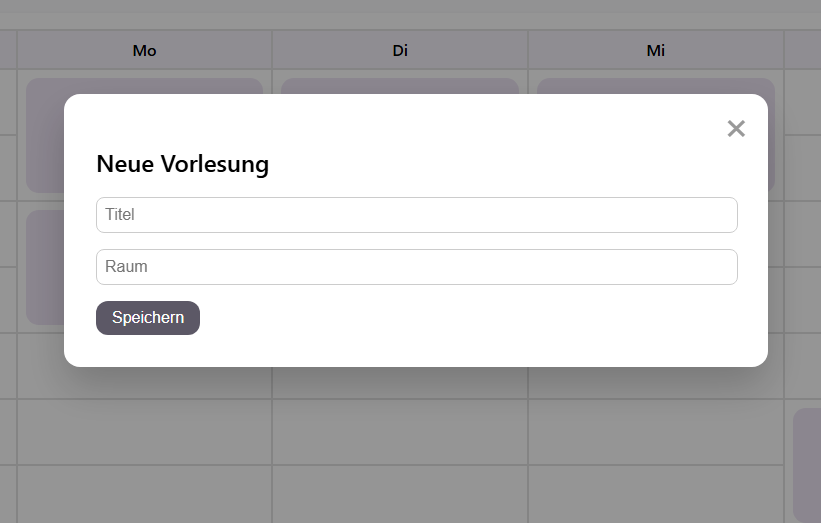
\includegraphics[width=1\textwidth]{./images/stundenplan-neuevorlesung.png}
  \caption{Neue Vorlesung hinzufügen}
  \label{fig:neue-vorlesungen}
\end{figure}

\begin{figure}[H]
  \centering
  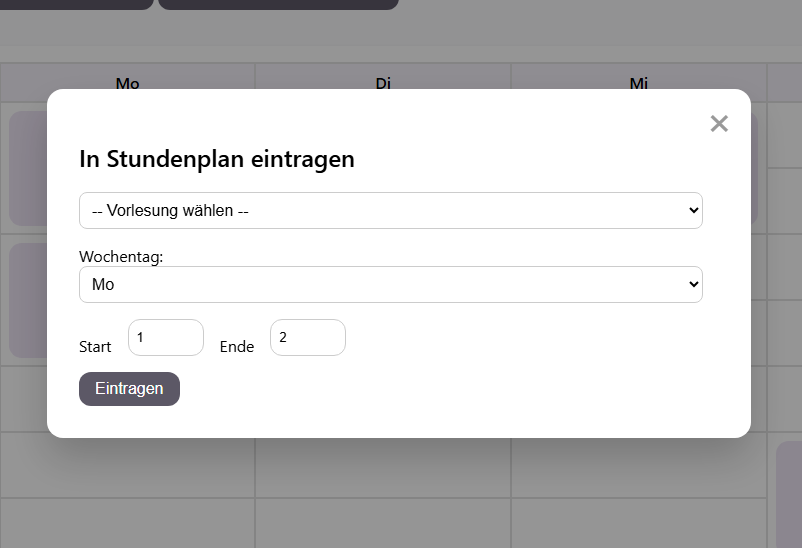
\includegraphics[width=1\textwidth]{./images/stundenplan-instundenplan.png}
  \caption{Vorlesung in den Stundenplan eintragen}
  \label{fig:stundenplan-vorlesung}
\end{figure}

Abbildung \ref{fig:stundenplan-vorlesungen} zeigt die Vorlesungsliste, in der alle verfügbaren Vorlesungen aufgelistet sind. Nutzer:innen können aus dieser Liste Vorlesungen löschen.
\begin{figure}[H]
  \centering
  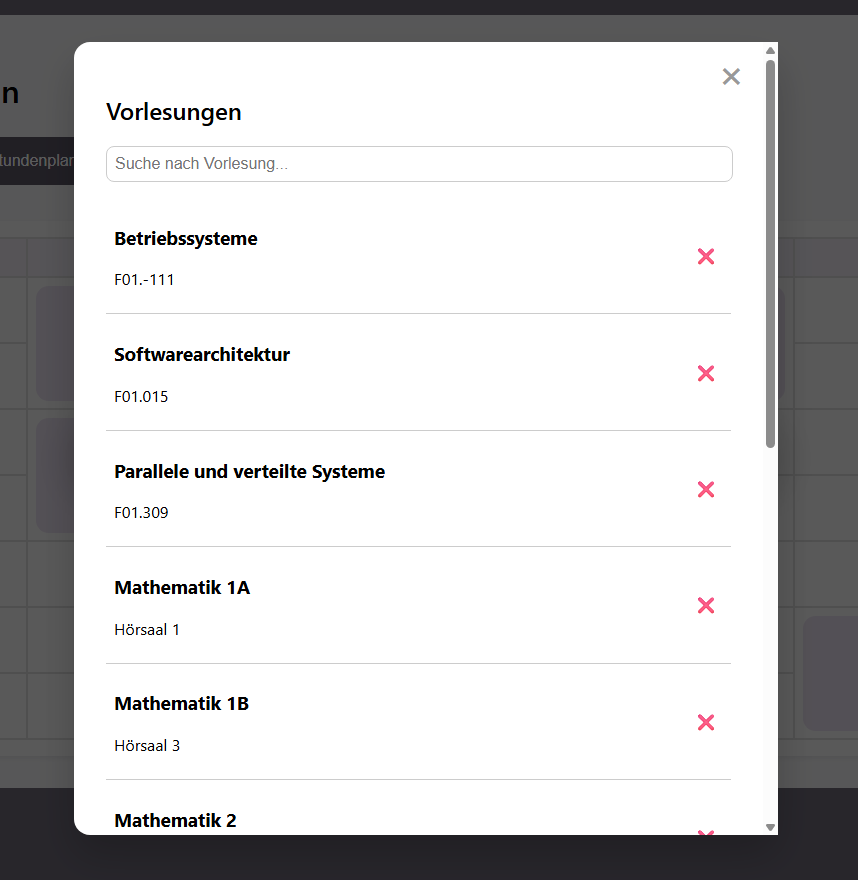
\includegraphics[width=1\textwidth]{./images/stundenplan-vorlesungsliste.png}
  \caption{Vorlesungsliste}
  \label{fig:stundenplan-vorlesungen}
\end{figure}

Die Web App bietet auch eine Notizfunktion, die es den Nutzer:innen ermöglicht, Notizen zu Vorlesungen zu erstellen und zu verwalten. In Abbildung \ref{fig:notizen} sind die Notizen und Lernmaterialien zu sehen, die hochgeladen und kategorisiert werden können. Nutzer:innen können Notizen zu spezifischen Vorlesungen hinzufügen und diese nach Bedarf organisieren.\newline
\begin{figure}[H]
  \centering
  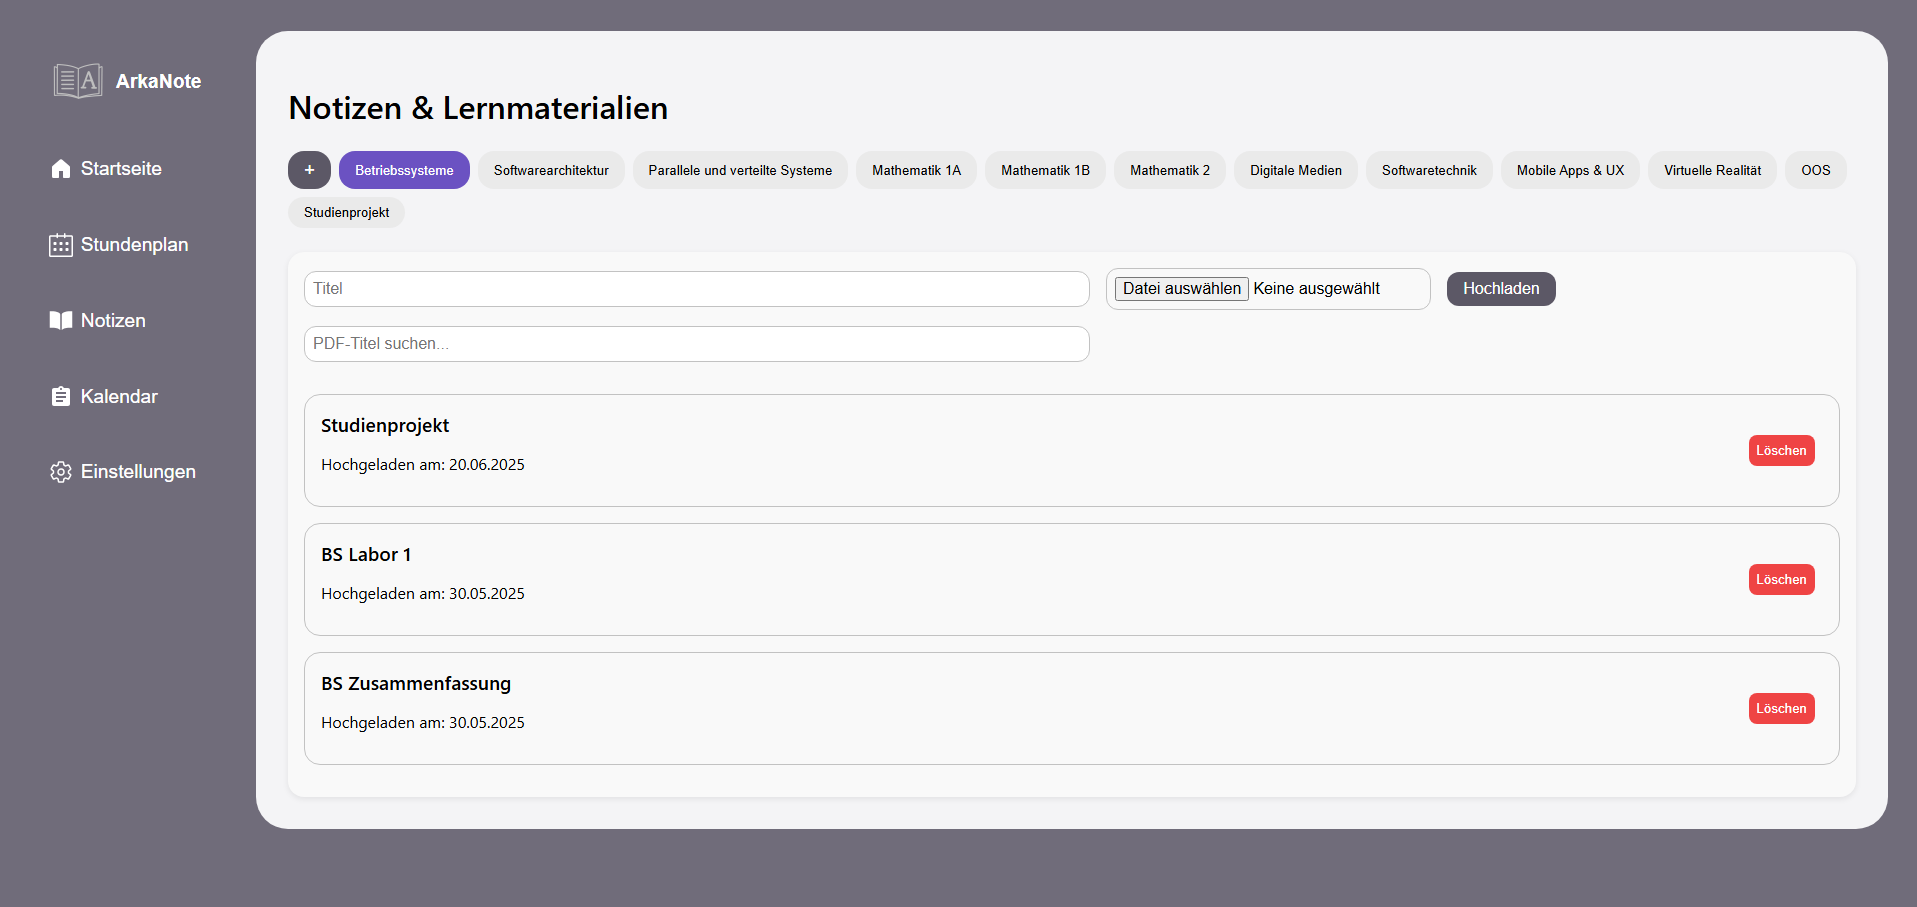
\includegraphics[width=1\textwidth]{./images/notizen.png}
  \caption{Notizen und Lernmaterialien}
  \label{fig:notizen}
\end{figure}

Die Kalenderfunktion der Web App ermöglicht es den Nutzer:innen, Termine und Fristen zu verwalten. In Abbildung \ref{fig:kalender} ist der Kalender zu sehen, in dem Nutzer:innen Ereignisse hinzufügen können, wie in Abbildung \ref{fig:kalender-ereignis} gezeigt. Diese Funktionalität ist besonders nützlich, um wichtige Termine im Blick zu behalten und eine bessere Organisation des Studienalltags zu ermöglichen.\newline
\begin{figure}[H]
  \centering
  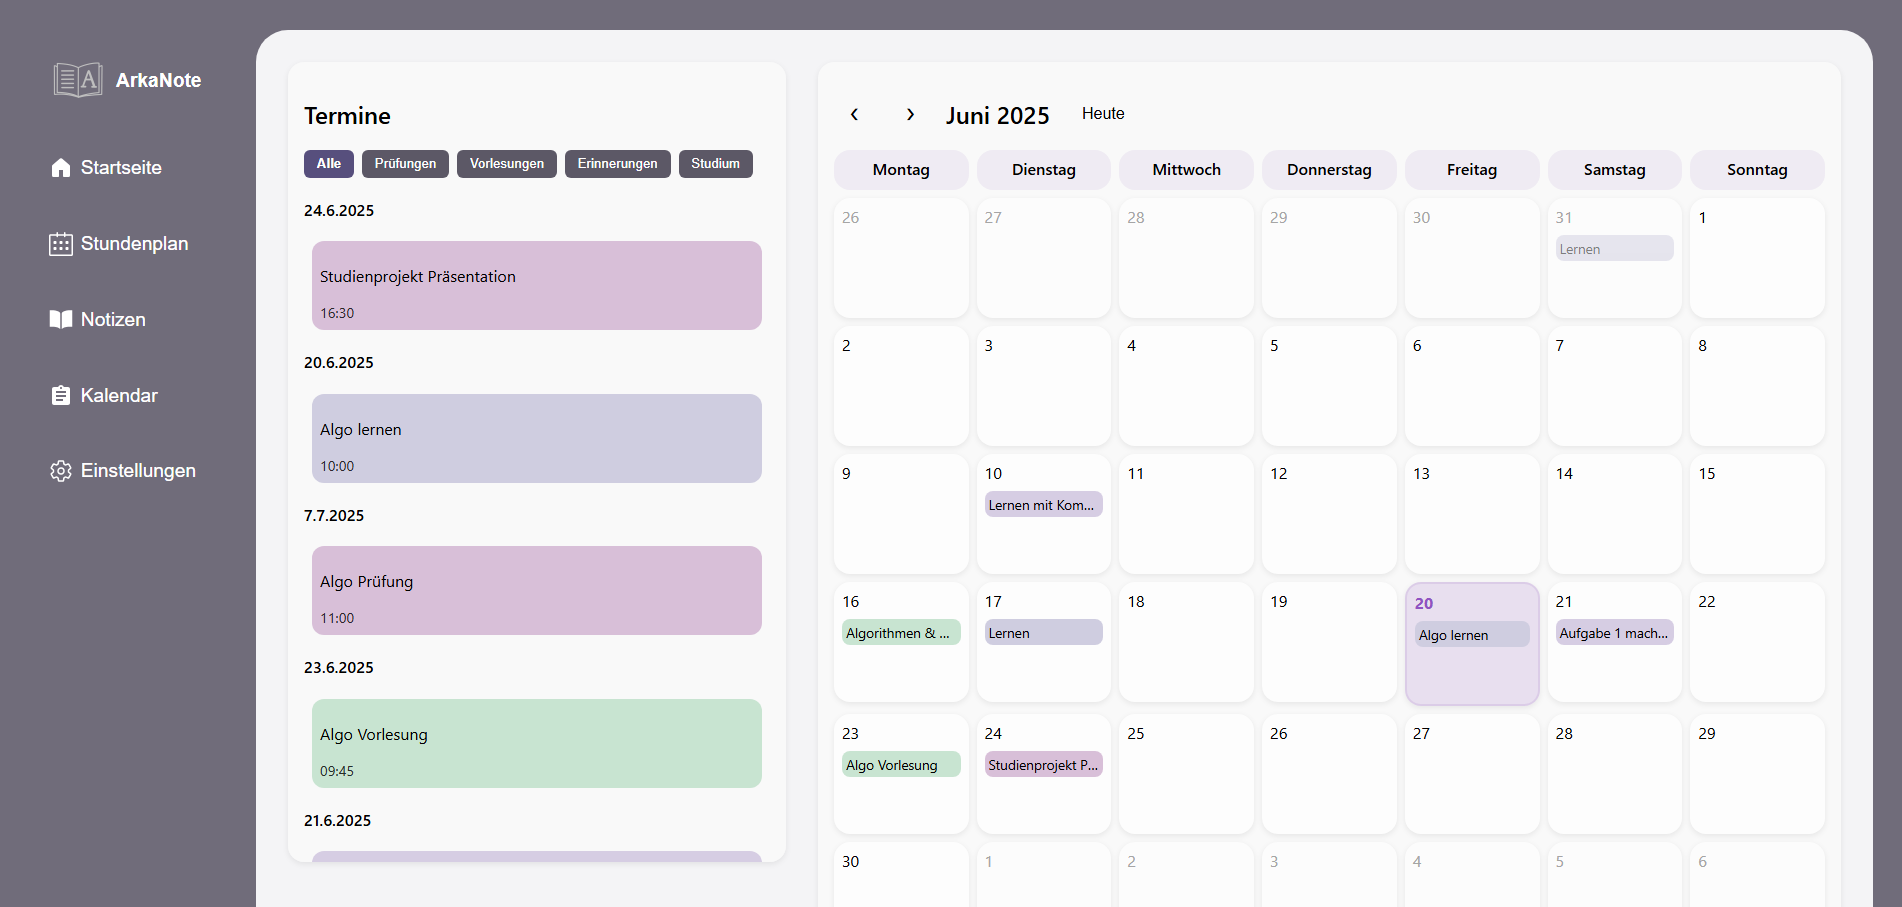
\includegraphics[width=1\textwidth]{./images/kalender.png}
  \caption{Kalender}
  \label{fig:kalender}
\end{figure}

\begin{figure}[H]
  \centering
  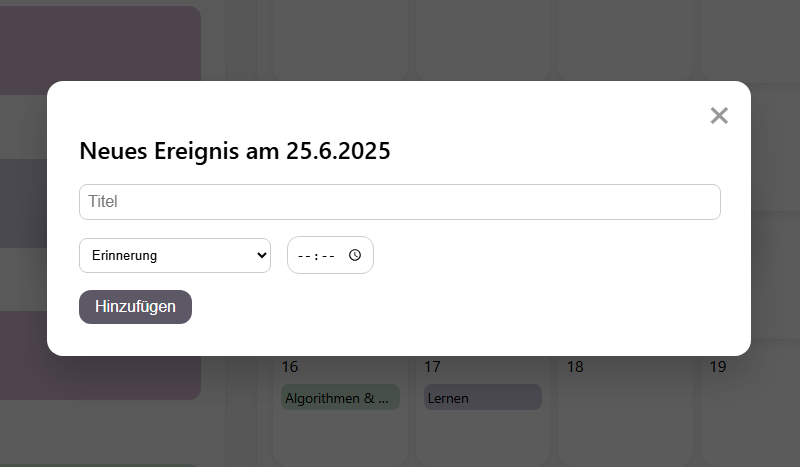
\includegraphics[width=1\textwidth]{./images/kalender-ereignis.png}
  \caption{Kalenderereignis hinzufügen}
  \label{fig:kalender-ereignis}
\end{figure}

Abbildung \ref{fig:einstellungen} zeigt die Einstellungen der Web App, in denen Nutzer:innen ihre persönlichen Daten verwalten und das Design der Anwendung anpassen können. \newline
\begin{figure}[H]
  \centering
  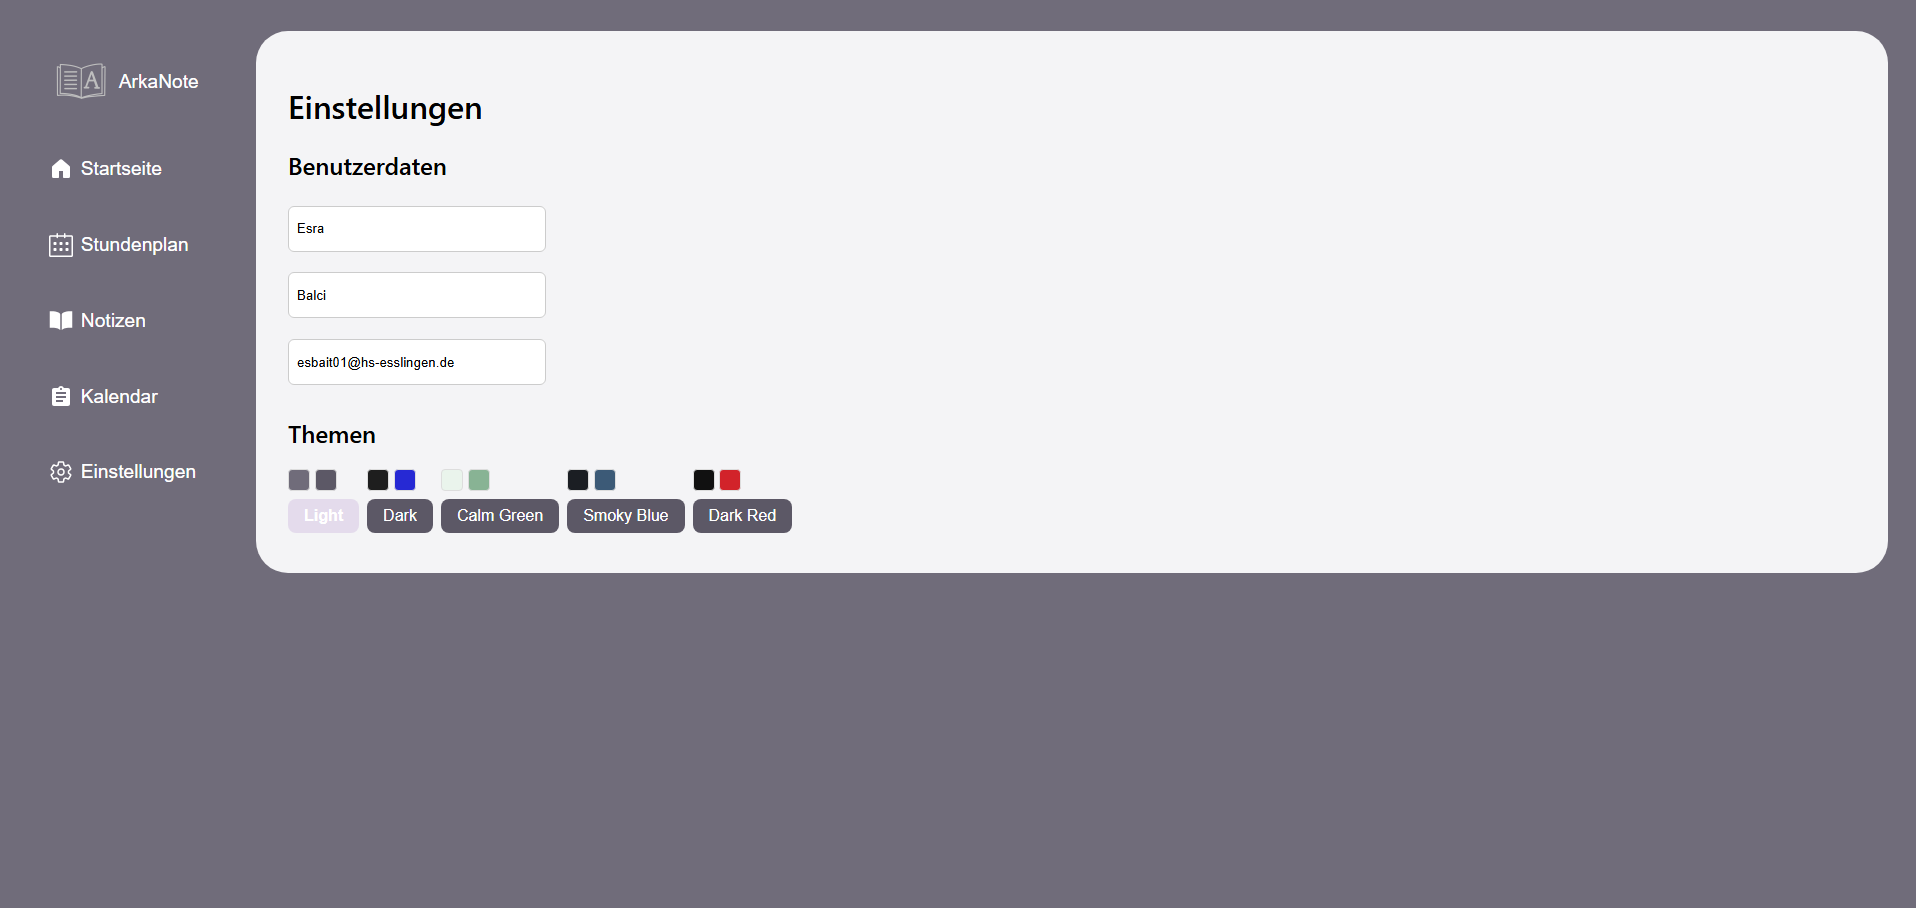
\includegraphics[width=1\textwidth]{./images/einstellungen.png}
  \caption{Einstellungen}
  \label{fig:einstellungen}
\end{figure}

Die Web App bietet verschiedene Design-Themes, die den Nutzer:innen eine individuelle Anpassung ermöglichen. In den Abbildungen \ref{fig:startseite-dark}, \ref{fig:kalender-dark}, \ref{fig:startseite-green}, \ref{fig:kalender-green}, \ref{fig:startseite-blue}, \ref{fig:kalender-blue}, \ref{fig:startseite-red} und \ref{fig:kalender-red} sind die verschiedenen Themes zu sehen, die den Nutzer:innen zur Verfügung stehen.\newline
\begin{figure}[H]
  \centering
  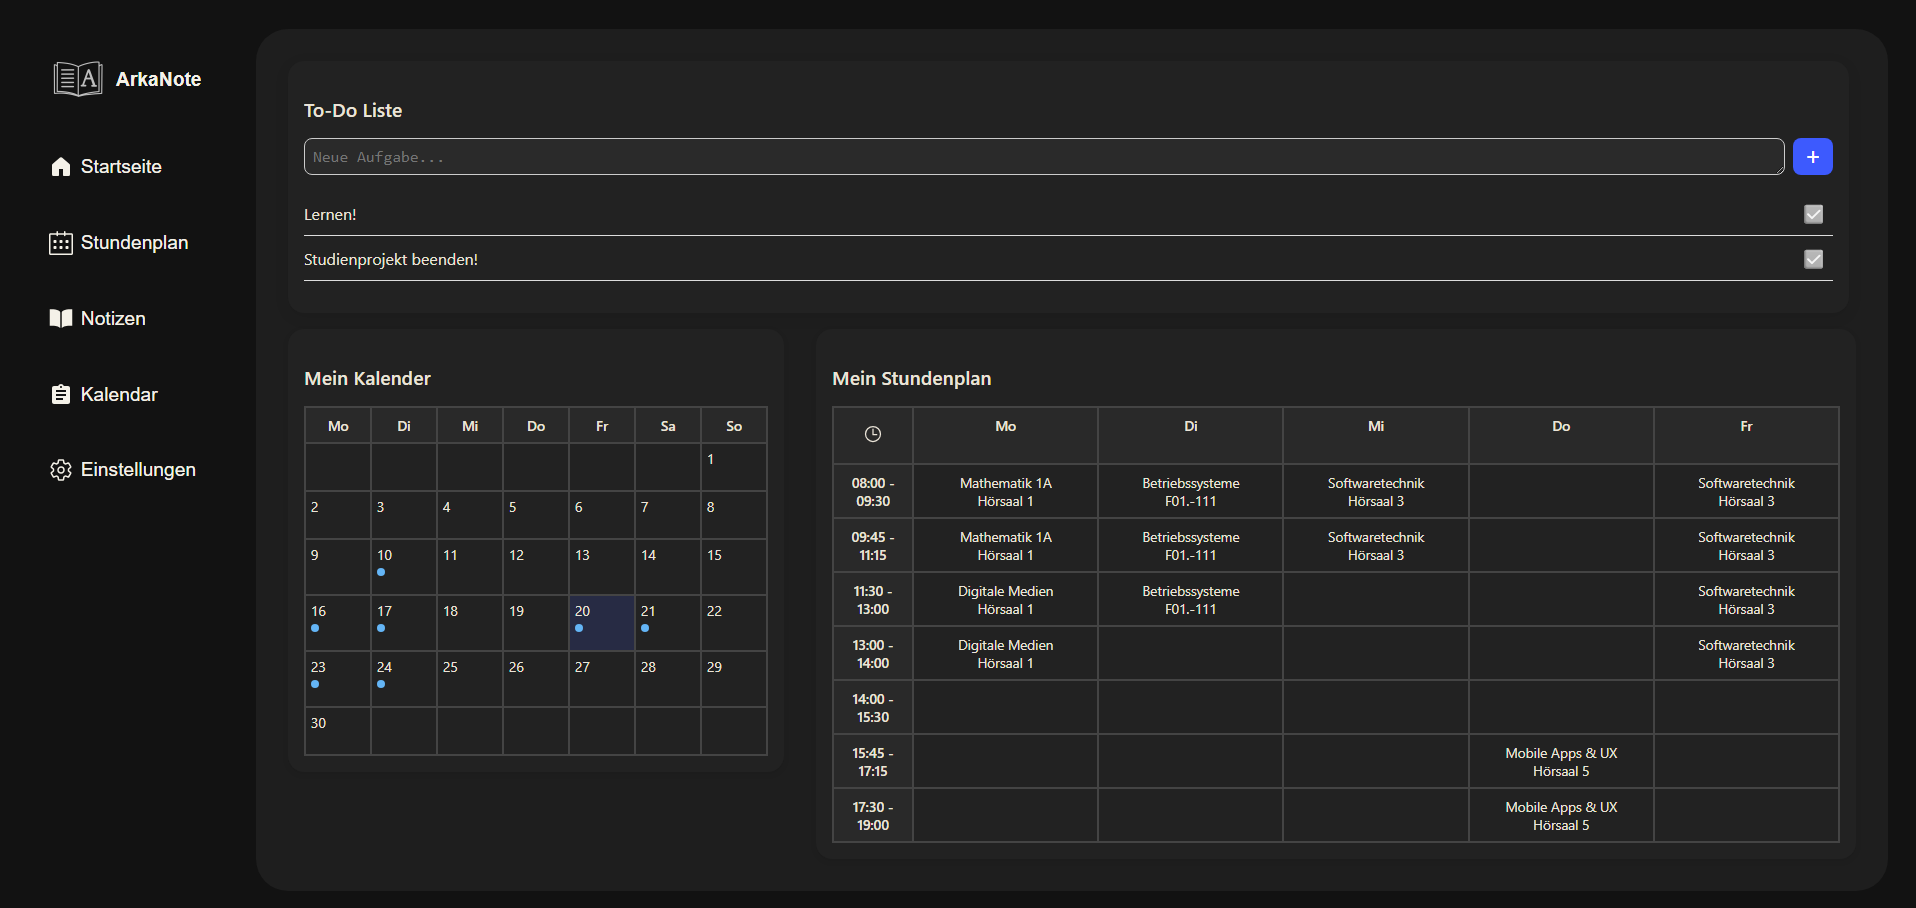
\includegraphics[width=1\textwidth]{./images/startseite-dark.png}
  \caption{Startseite im Dark Theme}
  \label{fig:startseite-dark}
\end{figure}

\begin{figure}[H]
  \centering
  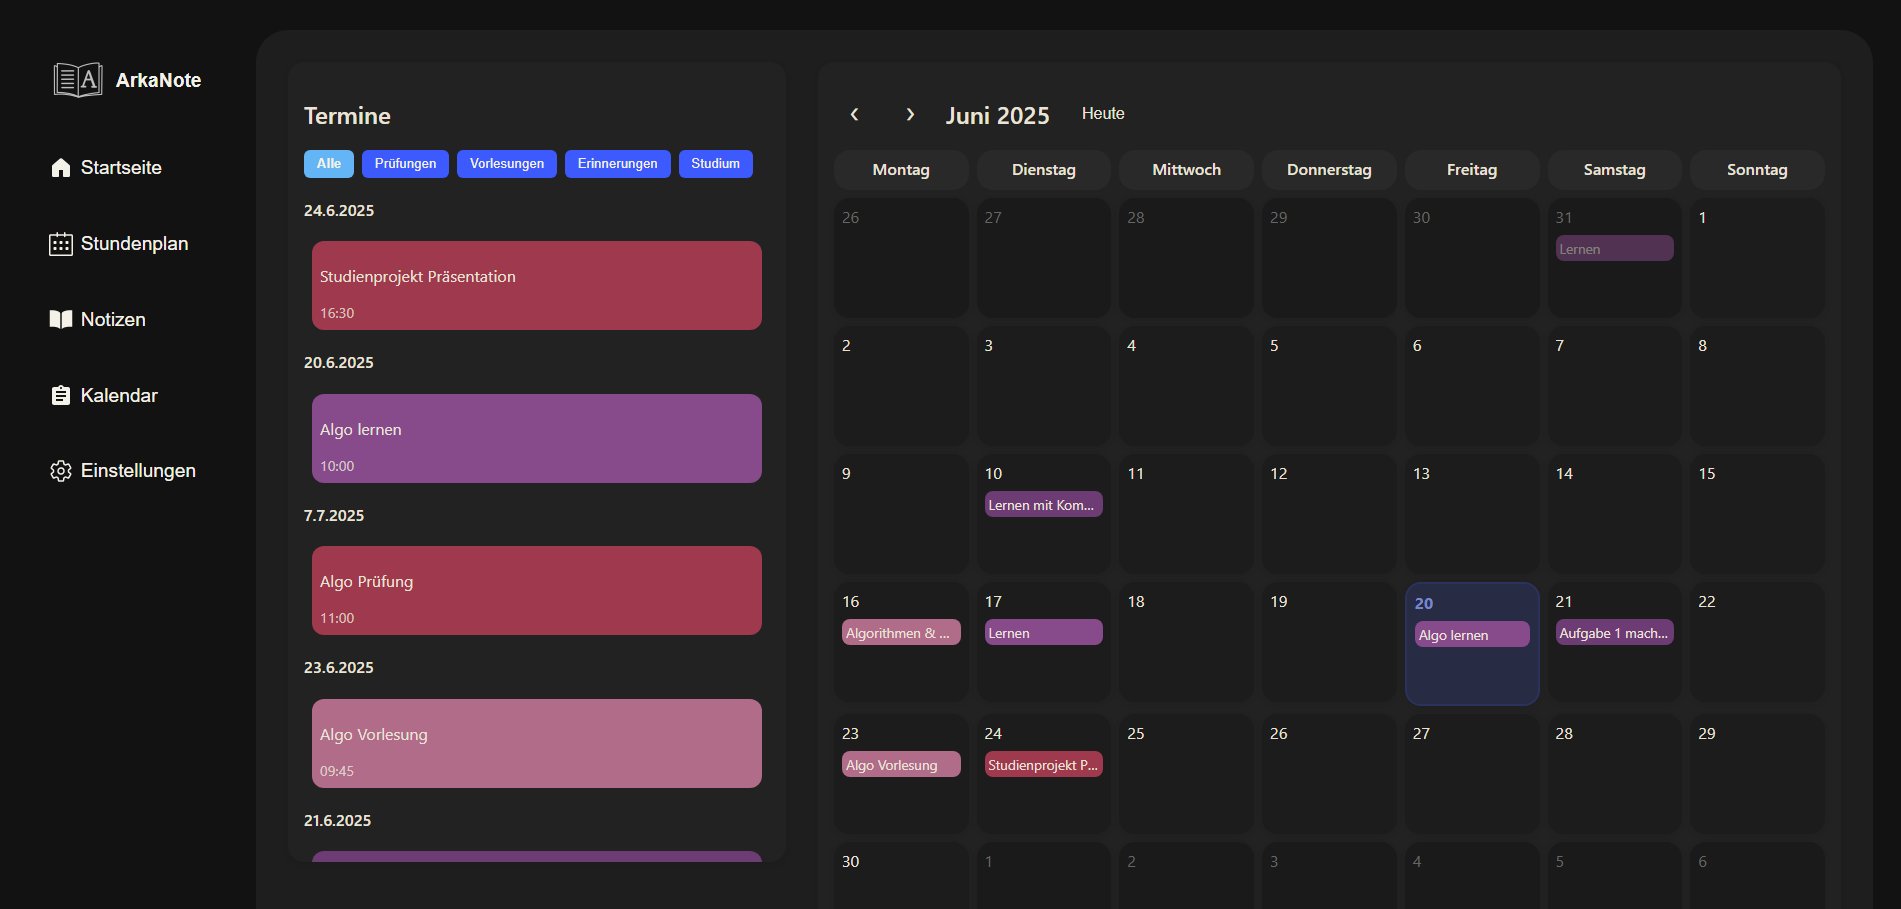
\includegraphics[width=1\textwidth]{./images/kalender-dark.png}
  \caption{Kalender im Dark Theme}
  \label{fig:kalender-dark}
\end{figure}

\begin{figure}[H]
  \centering
  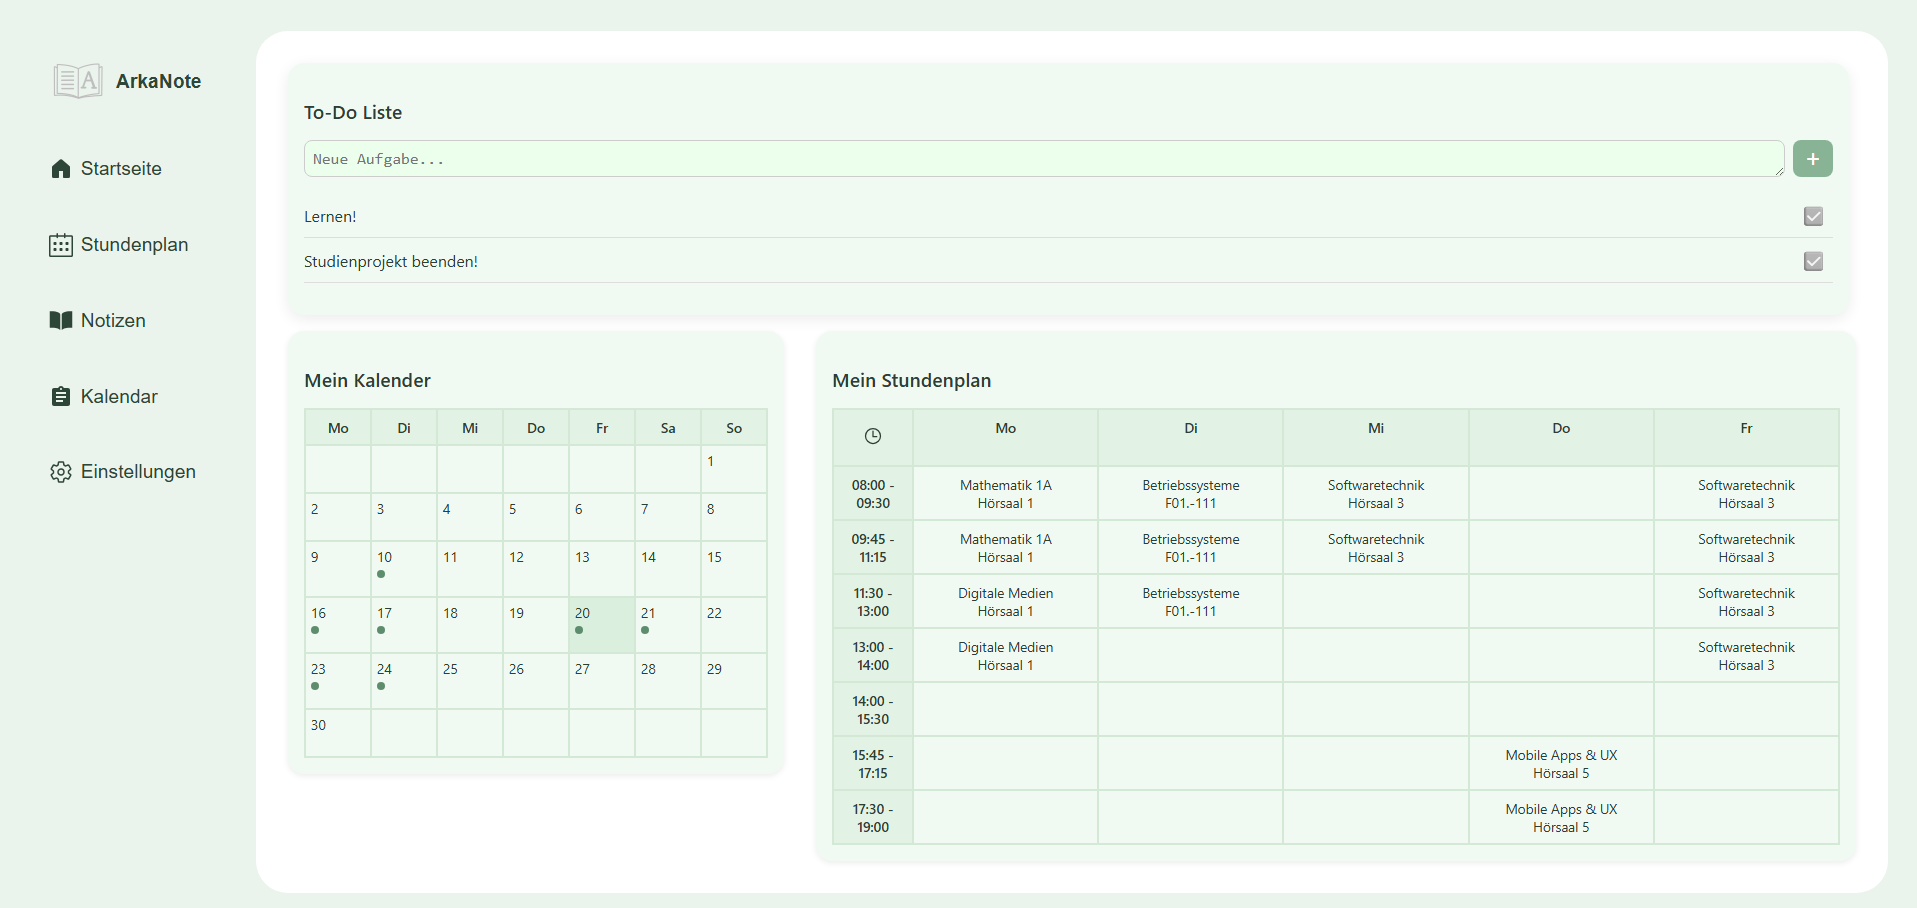
\includegraphics[width=1\textwidth]{./images/startseite-green.png}
  \caption{Startseite im Calm Green Theme}
  \label{fig:startseite-green}
\end{figure}

\begin{figure}[H]
  \centering
  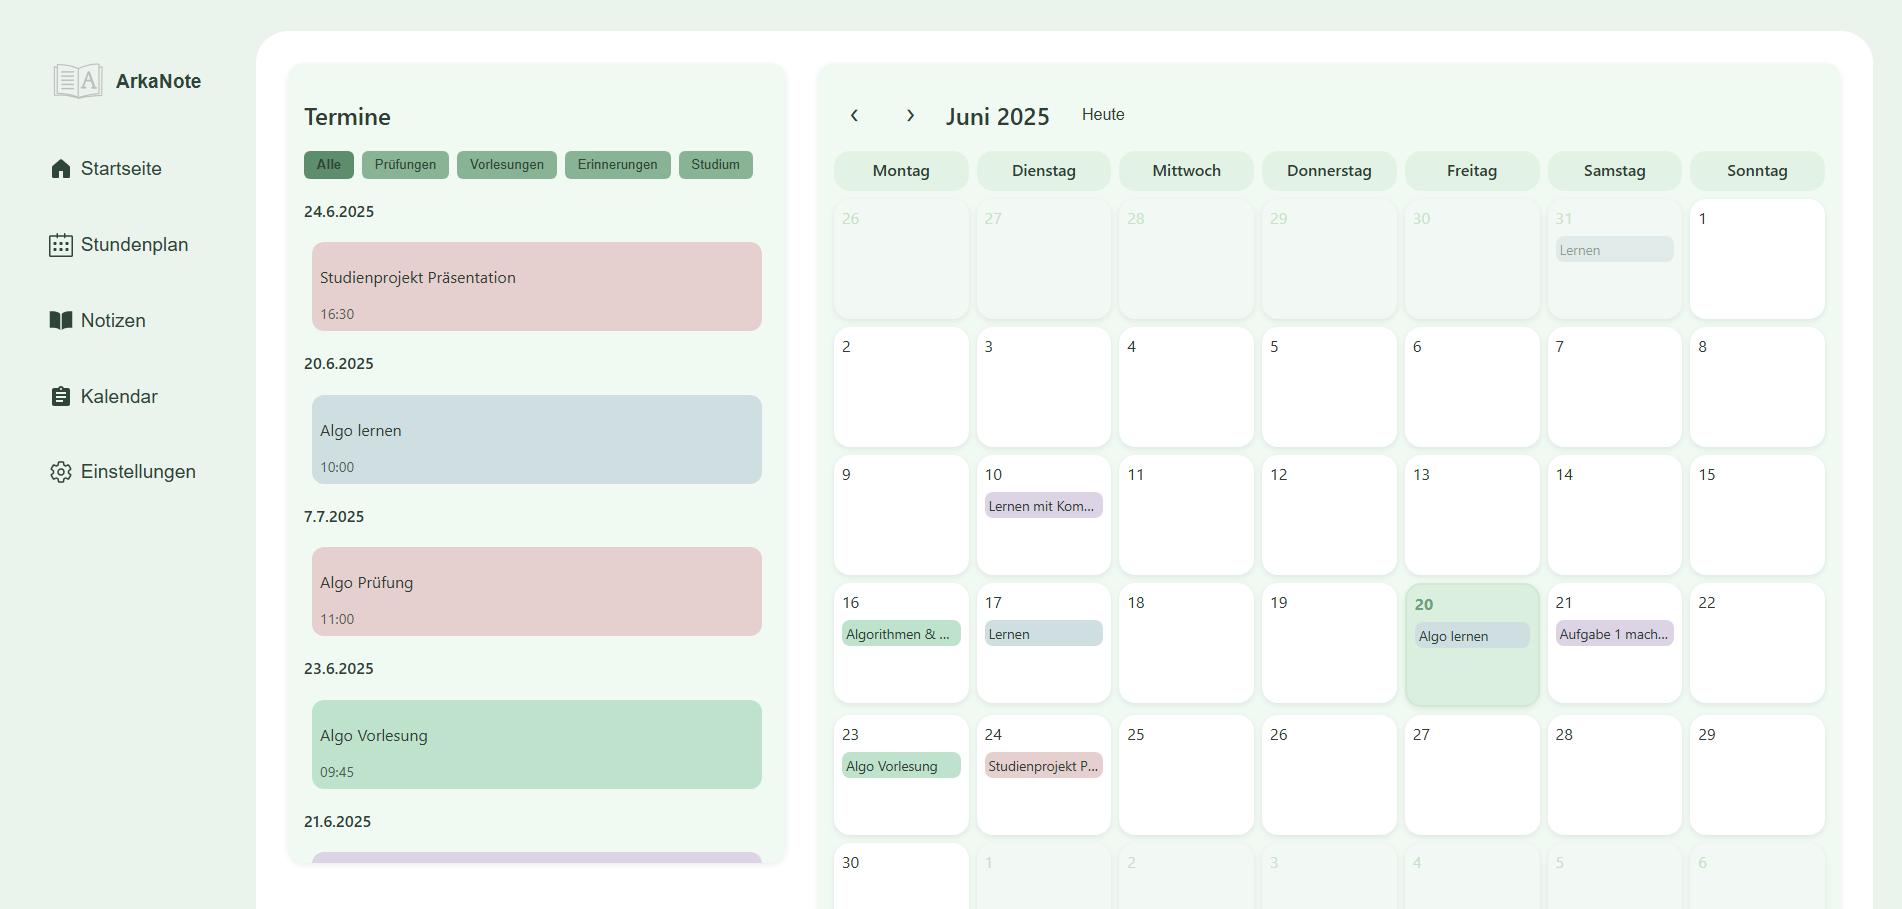
\includegraphics[width=1\textwidth]{./images/kalender-green.png}
  \caption{Kalender im Calm Green Theme}
  \label{fig:kalender-green}
\end{figure}

\begin{figure}[H]
  \centering
  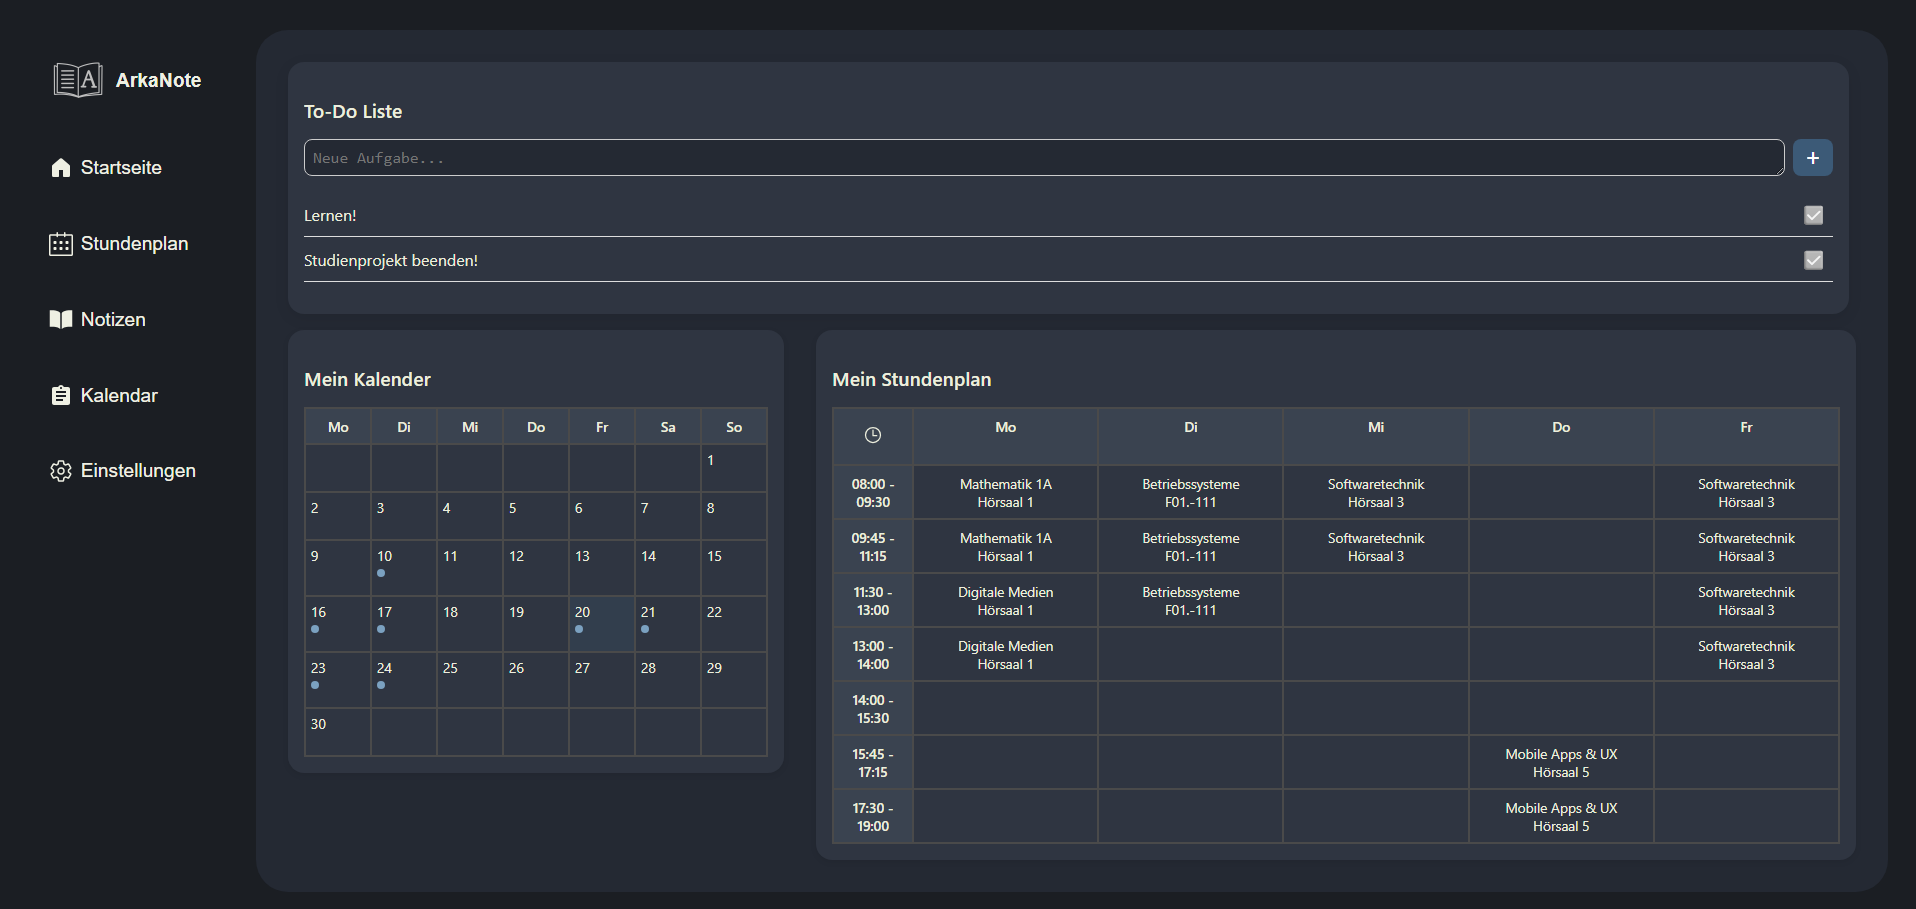
\includegraphics[width=1\textwidth]{./images/startseite-blue.png}
  \caption{Startseite im Smoky Blue Theme}
  \label{fig:startseite-blue}
\end{figure}

\begin{figure}[H]
  \centering
  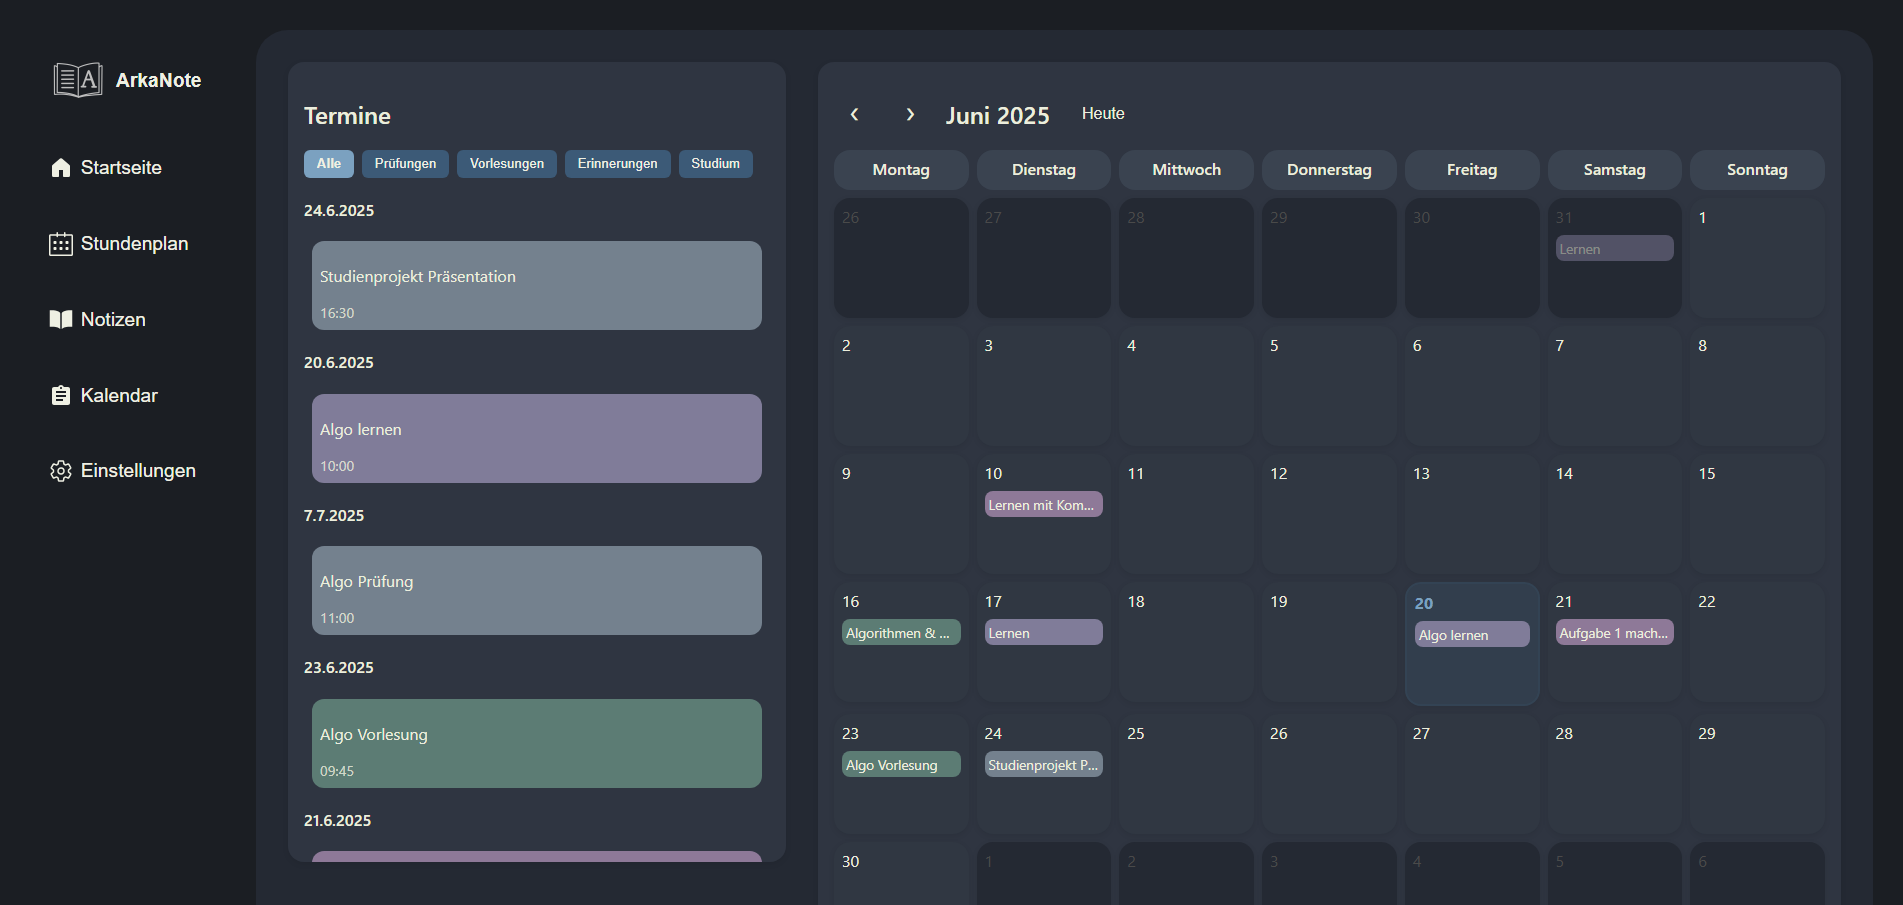
\includegraphics[width=1\textwidth]{./images/kalender-blue.png}
  \caption{Kalender im Smoky Blue Theme}
  \label{fig:kalender-blue}
\end{figure}

\begin{figure}[H]
  \centering
  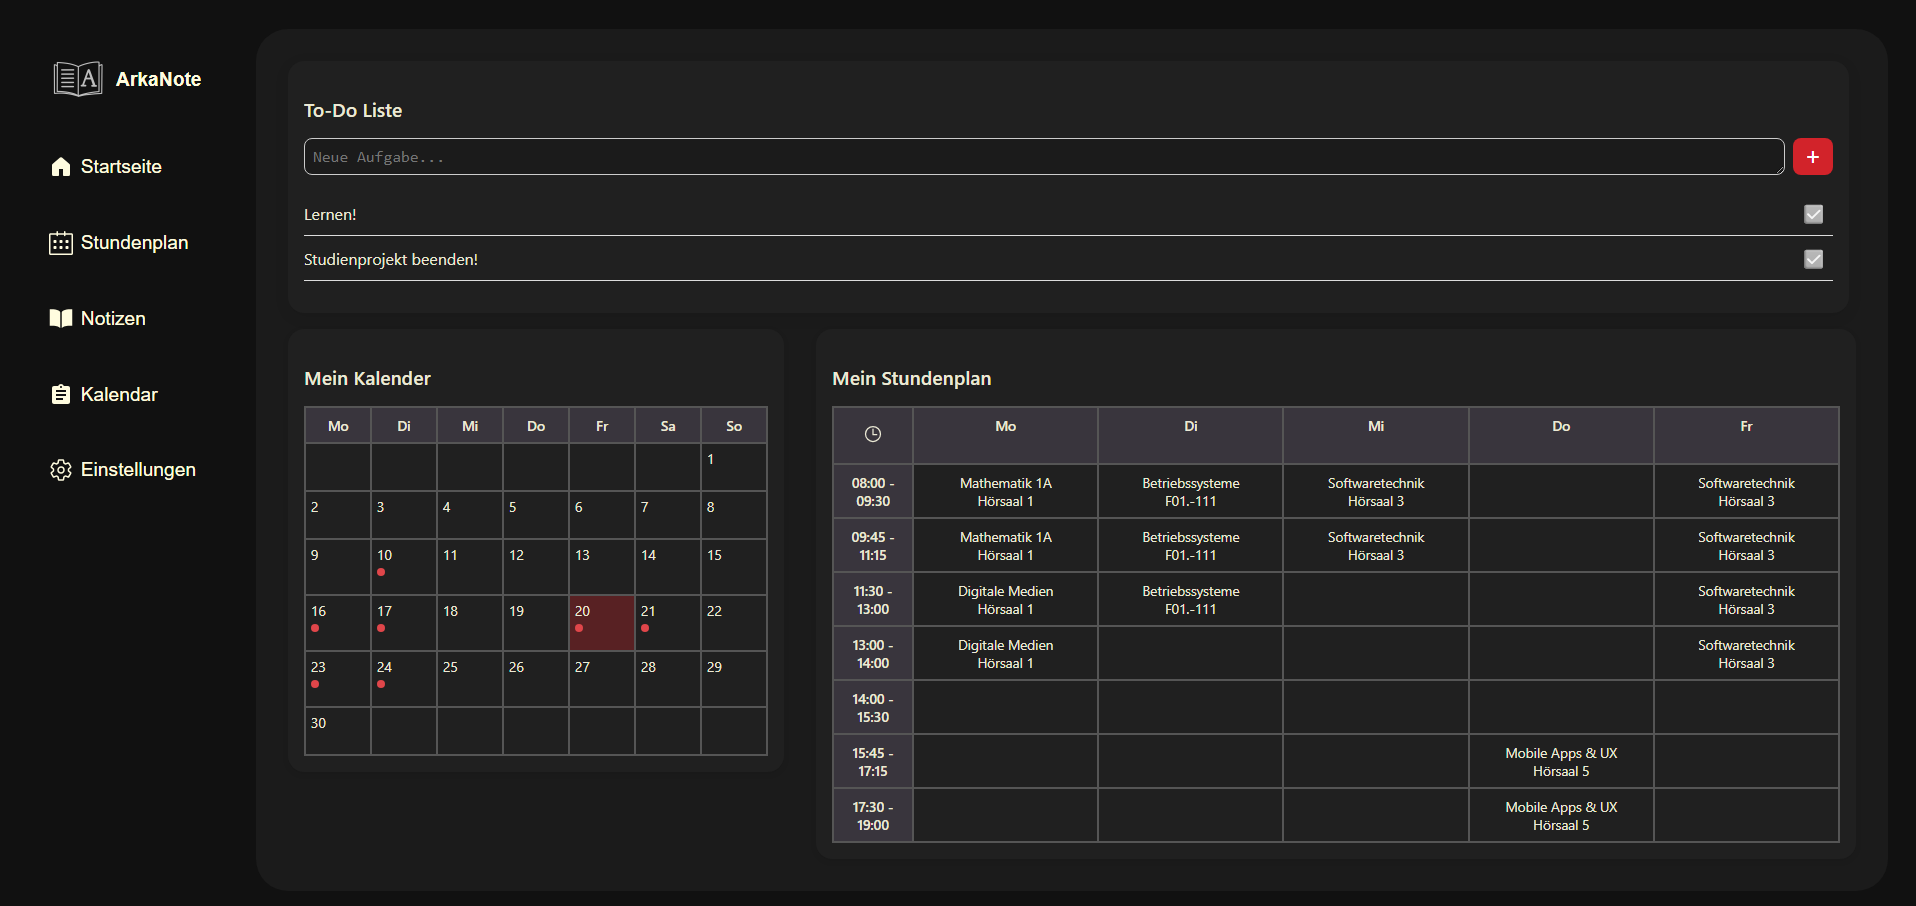
\includegraphics[width=1\textwidth]{./images/startseite-red.png}
  \caption{Startseite im Dark Red Theme}
  \label{fig:startseite-red}
\end{figure}

\begin{figure}[H]
  \centering
  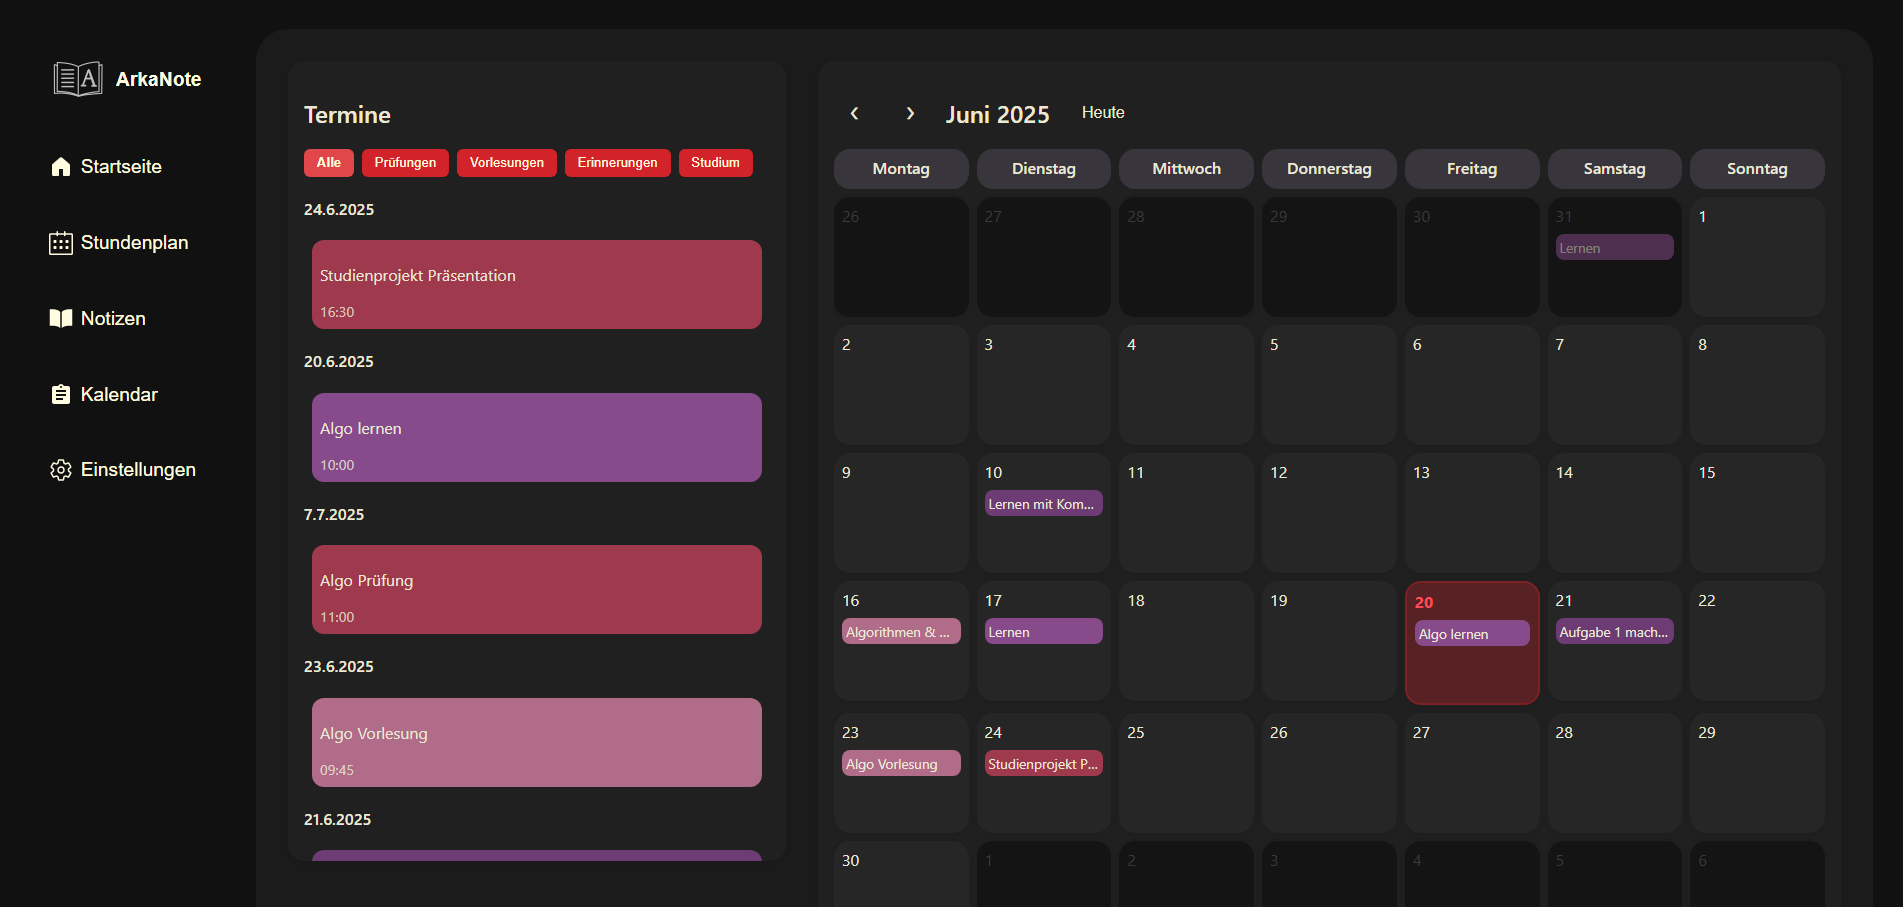
\includegraphics[width=1\textwidth]{./images/kalender-red.png}
  \caption{Kalender im Dark Red Theme}
  \label{fig:kalender-red}
\end{figure}

\section{Vergleich zu bestehenden Lösungen}
\begin{table}[H]
\centering
\scriptsize % kleinere Schriftgröße für bessere Lesbarkeit
\renewcommand{\arraystretch}{1.3} % etwas mehr Zeilenhöhe
\begin{tabularx}{\textwidth}{|p{3cm}|p{2.3cm}|p{2.5cm}|p{2.5cm}|p{2.5cm}|}
\hline
\textbf{Kriterium / Tool} & \textbf{Projekt} & \textbf{Moodle} & \textbf{Google Kalender} & \textbf{Notion} \\
\hline
Zielgruppe & Studierende, selbstorganisiert & Hochschulen, Lehrende + Studis & Allgemein, breites Publikum & Teams, Selbstorganisation \\
\hline
Stundenplan-Funktion & Visuell und interaktiv & Nicht enthalten & Nur Ereignisse & Manuell möglich \\
\hline
Kalender & Mit Deadlines und Kategorien & Mit Farbcodes + Kategorien & Eingeschränkt, wenig UX & Sehr leistungsfähig, aber unstrukturiert \\
\hline
Notizen mit Tags & Uploads & PDF-Upload + Tagging & Nur in Foren/Dateien & Sehr stark (Rich Content) \\
\hline
Offline-Funktion (PWA) & Nein & Nein & Nur mit Google Workspace & Nur mit App \\
\hline
Gebrauchstauglichkeit (UI) & Modern, Studierendenfokus & Veraltet, überladen & Klar und bekannt & Flexibel, aber komplex \\
\hline
Plattformunabhängigkeit & Web + App & Web + App & Web + App & Web + App \\
\hline
Open Source / Anpassbar & Ja (Eigenentwicklung möglich) & Teilweise & Nein & Nein \\
\hline
Integration in Lernumgebung & Manuell über Nutzung & Hochschulweit integriert & Nur externe Anbindung & Nur Copy/Paste \\
\hline
\end{tabularx}
\caption{Vergleich vom Projekt mit bestehenden Tools für studentisches Selbstmanagement}
\label{tab:toolvergleich}
\end{table}



\section{Offene Punkte und mögliche Erweiterungen}
Die entwickelte Web App erfüllt grundlegende Anforderungen an ein digitales Selbstorganisationswerkzeug, weist jedoch in ihrer aktuellen Version noch einige funktionale und technische Lücken auf, die in zukünftigen Entwicklungsschritten adressiert werden sollten.\newline 
Derzeit besteht keine Möglichkeit zur geräteübergreifenden Synchronisation von Daten. Dies bedeutet dass die Nutzung auf ein einzelnes Gerät beschränkt bleibt. Eine logische Weiterentwicklung stellt die Einführung eines cloudbasierten Backends mit Benutzerverwaltung dar.\newline 
Zudem fehlen Push-Benachrichtigungen, die die Nutzer:innen aktiv an bevorstehende Termine und Fristen erinnern könnten. Die Integration solcher Erinnerungsfunktionen würde den Nutzwert der App im Studienalltag deutlich steigern, insbesondere in Verbindung mit der Kalenderfunktion.\newline 
Neben der technischen Weiterentwicklung bestehen auch funktionale Erweiterungspotenziale. So wäre beispielsweise die Unterstützung von Gruppenfunktionen denkbar, bei der Studierende gemeinsame Notizen verwalten oder Termine in Lerngruppen organisieren können. Dies würde die Web App auch für kollaborative Lernszenarien attraktiver machen.\newline 
Langfristig ließe sich die Anwendung zudem durch den Einsatz Künstlicher Intelligenz erweitern. Möglich wären beispielsweise automatische Zusammenfassungen von Notizen oder intelligente Vorschläge für die Terminplanung auf Basis individueller Lernmuster. Diese Erweiterungen könnten nicht nur die Effizienz der Web App steigern, sondern auch den indiviuellen Lernprozess der Studierenden nachhaltig fördern.
% \chapter{Deployment}
Dieses Kapitel beschreibt die notwendigen Schritte zur Bereitstellung der entwickelten Webanwendung. 
\begin{enumerate}
    \item Klonen Sie das GitHub Repository:\newline
    \texttt{git clone https://github.com/sheg0/studienprojekt.git}
    \item Wechseln Sie in das Verzeichnis des Projekts:\newline
    \texttt{cd studienprojekt}
    \item Installieren Sie die Abhängigkeiten für das Backend:\newline
    \texttt{cd backend}\newline
    \texttt{npm install}
    \item Pullen Sie Docker:\newline
    \texttt{docker pull shego/backend-backend}
    \item Installieren Sie die Abhängigkeiten für das Frontned:\newline
    \texttt{cd ../frontend}\newline
    \texttt{npm install}
    \item Starten Sie alle Services im Backend über Docker Compose:\newline
    \texttt{docker-compose up --build}
    \item Starten Sie das Frontend:\newline
    \texttt{npm start}
    \item Die Anwendung ist nun erreichbar unter:\newline
    \texttt{http://localhost:3000}
\end{enumerate}
\chapter{Fazit}

In dieser Arbeit wurde eine Progressive Web App (PWA) entwickelt und umgesetzt, die Studierenden bei der Organisation ihres Studienalltags unerstützt. Ziel war es, eine gebrauchstaugliche Oberfläche für Vorlesungen, Notizen und Prüfungstermine bereitzustellen.\newline 
Die Implementierung zeigt, dass mit modernen Webtechnologien wie ReactJS ein hoher Grad an Gebrauchstauglichkeit und Plattformunabhängigkeit erreicht werden kann. \newline
Für die Zukunft wären Features wie eine KI-gesstützte Zusammenfassung von Notizen oder eine Gruppenfunktion zur gemeinsamen Vorlesungsvorbereitung denkbar. Auch die Erweiterung auf eine native App oder die Integration in bestehende Hochschulplattformen bietet Potenzial.

\cleardoublepage
\phantomsection
\printbibliography[heading=bibintoc]

\end{document}
